\documentclass[tikz, border=0pt]{standalone}
\usepackage{graphicx}
\usepackage{tikz}

\usepackage{helvet}
\renewcommand{\familydefault}{\sfdefault}

\begin{document}
	\begin{tikzpicture}
		% DWI - slice0
		\node[font=\tiny] at (0.45, 1.6) {DWI};
		\node[font=\tiny] at (0.40, 1.3) {[$x$,~$y$,~$z$,~$q$]};

		\node[inner sep=0pt] (DWI-slice0-dir0) at (.45,.45)
		{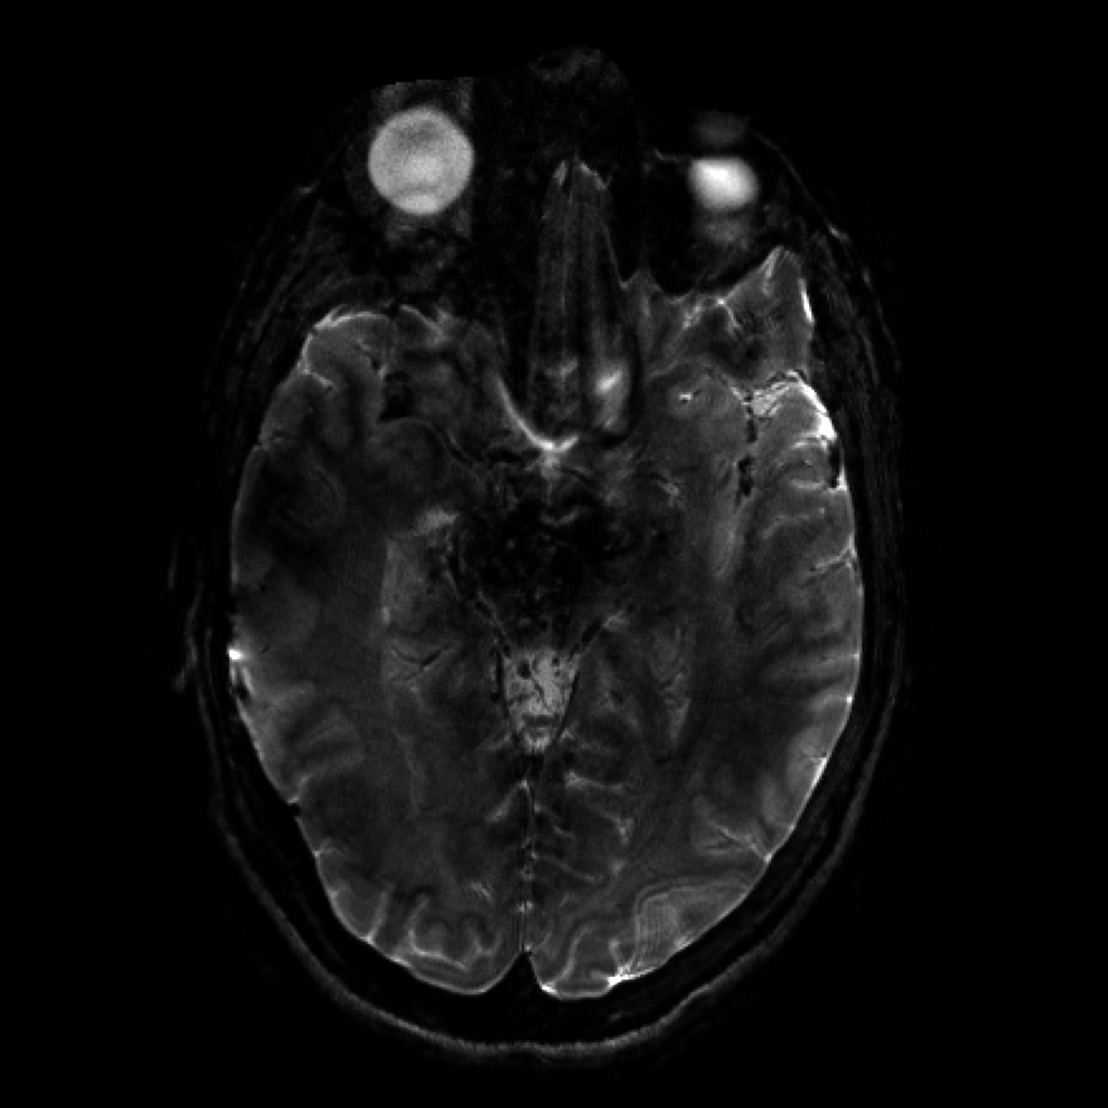
\includegraphics[width=.10\textwidth]{figures/DWI_dir-0_slice-0.png}};

		\node[inner sep=0pt] (DWI-slice0-dir3) at (.30,.30)
		{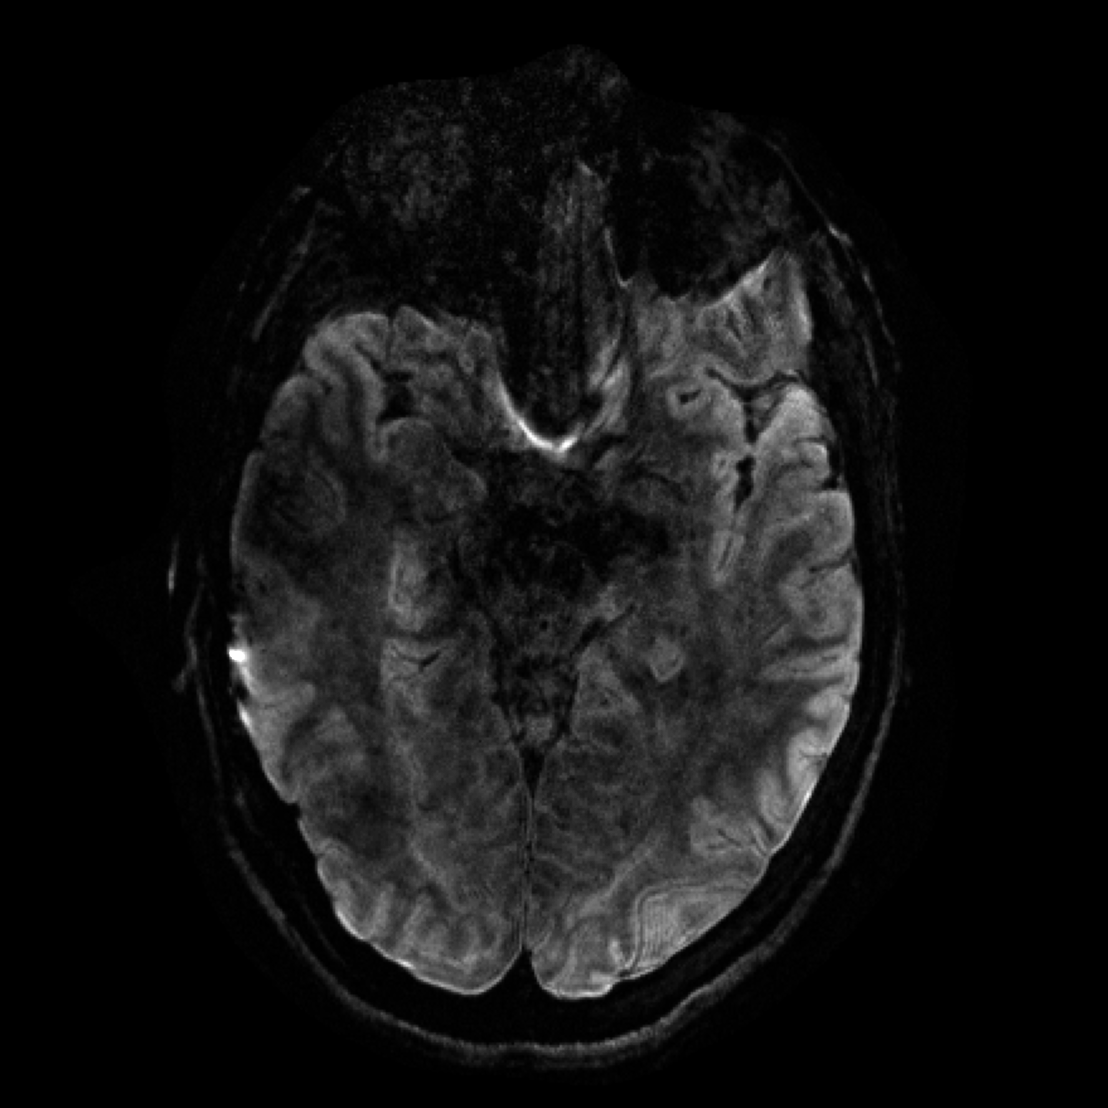
\includegraphics[width=.10\textwidth]{figures/DWI_dir-3_slice-0.png}};

		\node[inner sep=0pt] (DWI-slice0-dir2) at (.15,.15)
		{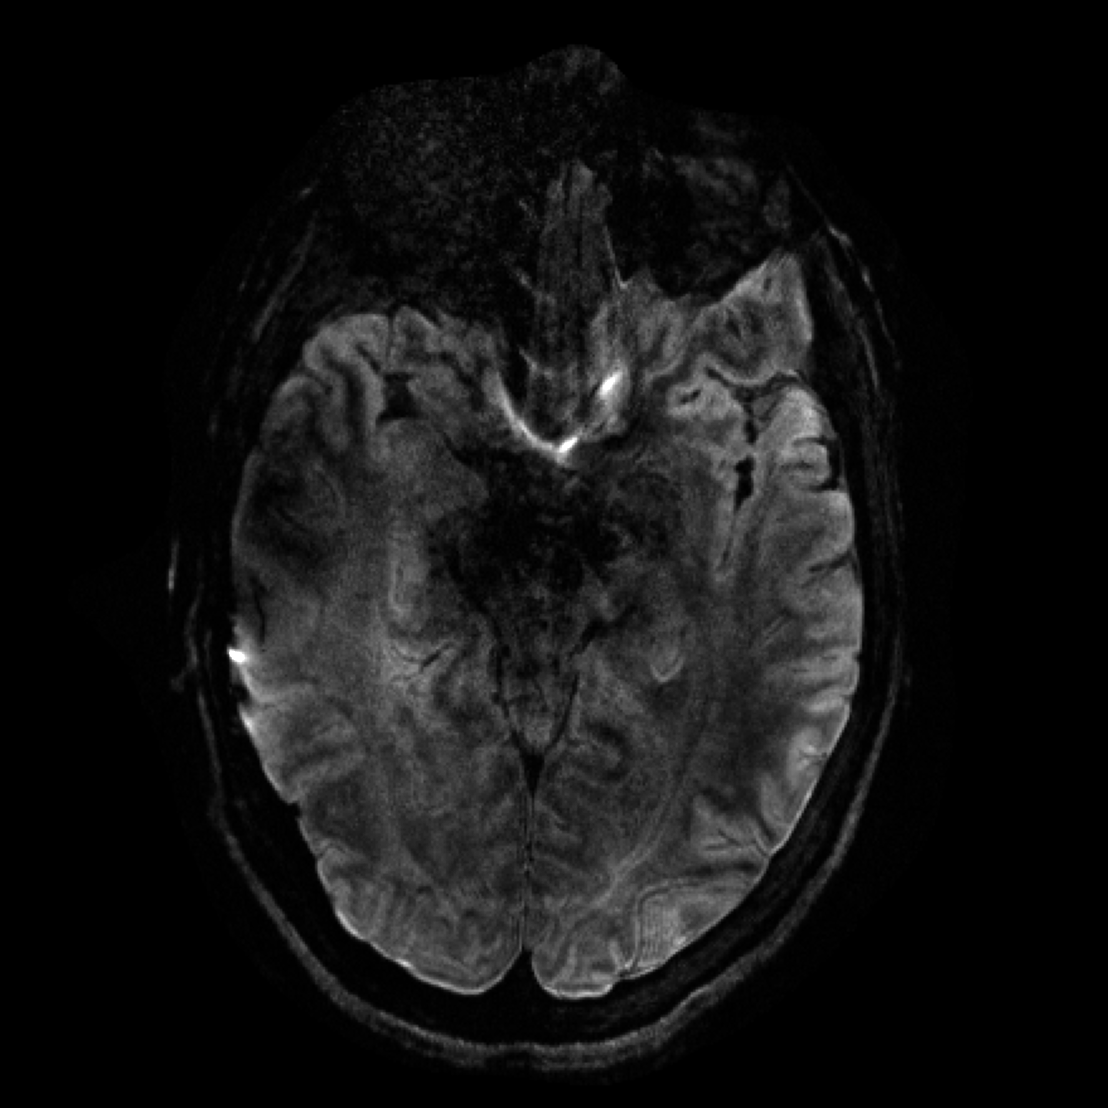
\includegraphics[width=.10\textwidth]{figures/DWI_dir-2_slice-0.png}};

		\node[inner sep=0pt] (DWI-slice0-dir1) at (0,0)
		{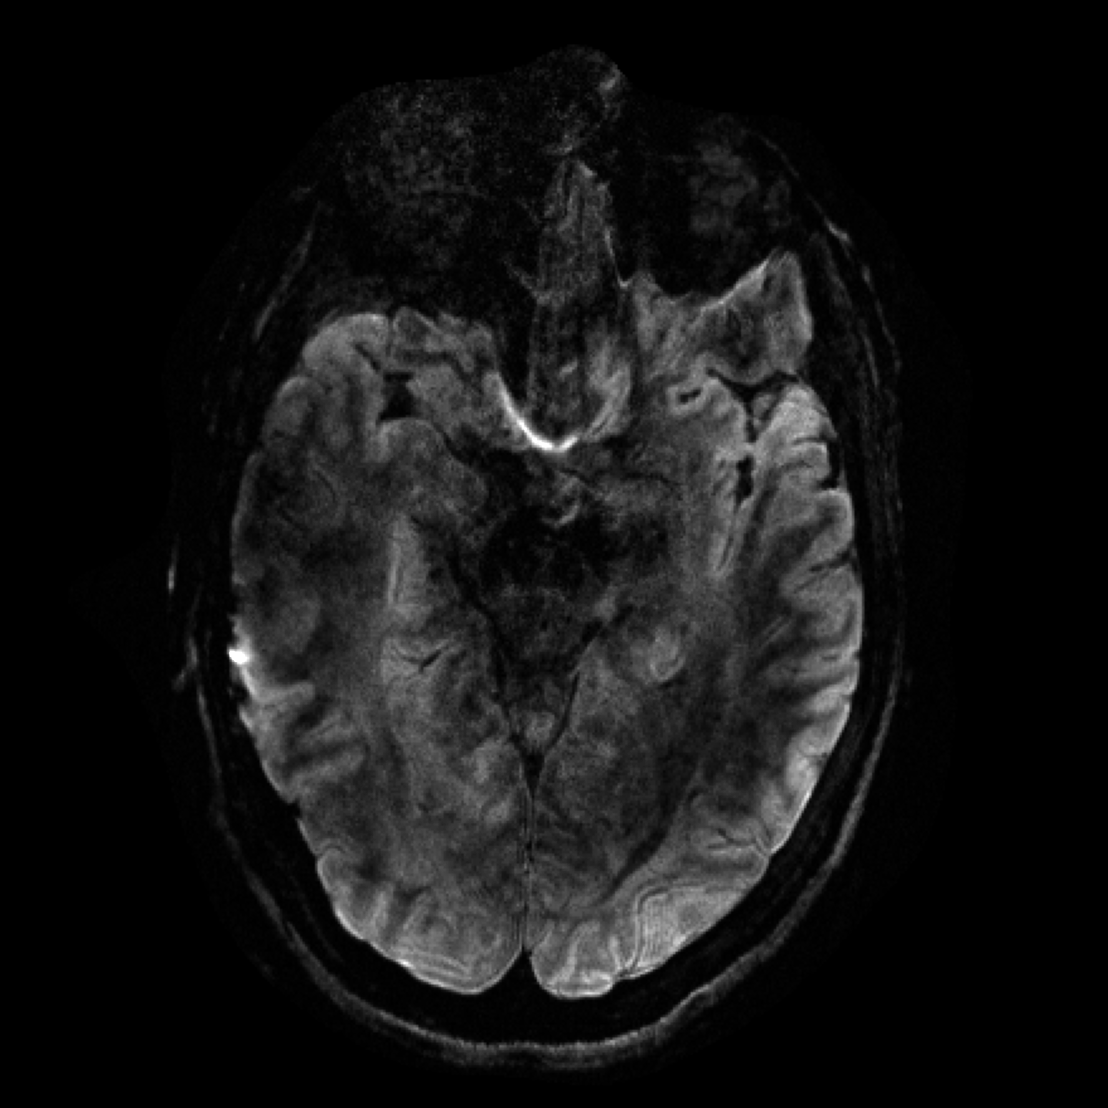
\includegraphics[width=.10\textwidth]{figures/DWI_dir-1_slice-0.png}};

		\draw[->, line width=0.5pt] (0.8, -0.5) -- (1.0, -0.3);
		\node[font=\tiny] at (1.05, -0.4) {$q$};

		% DWI - slice1
		\node[inner sep=0pt] (DWI-slice1-dir0) at (.45, -1.55)
		{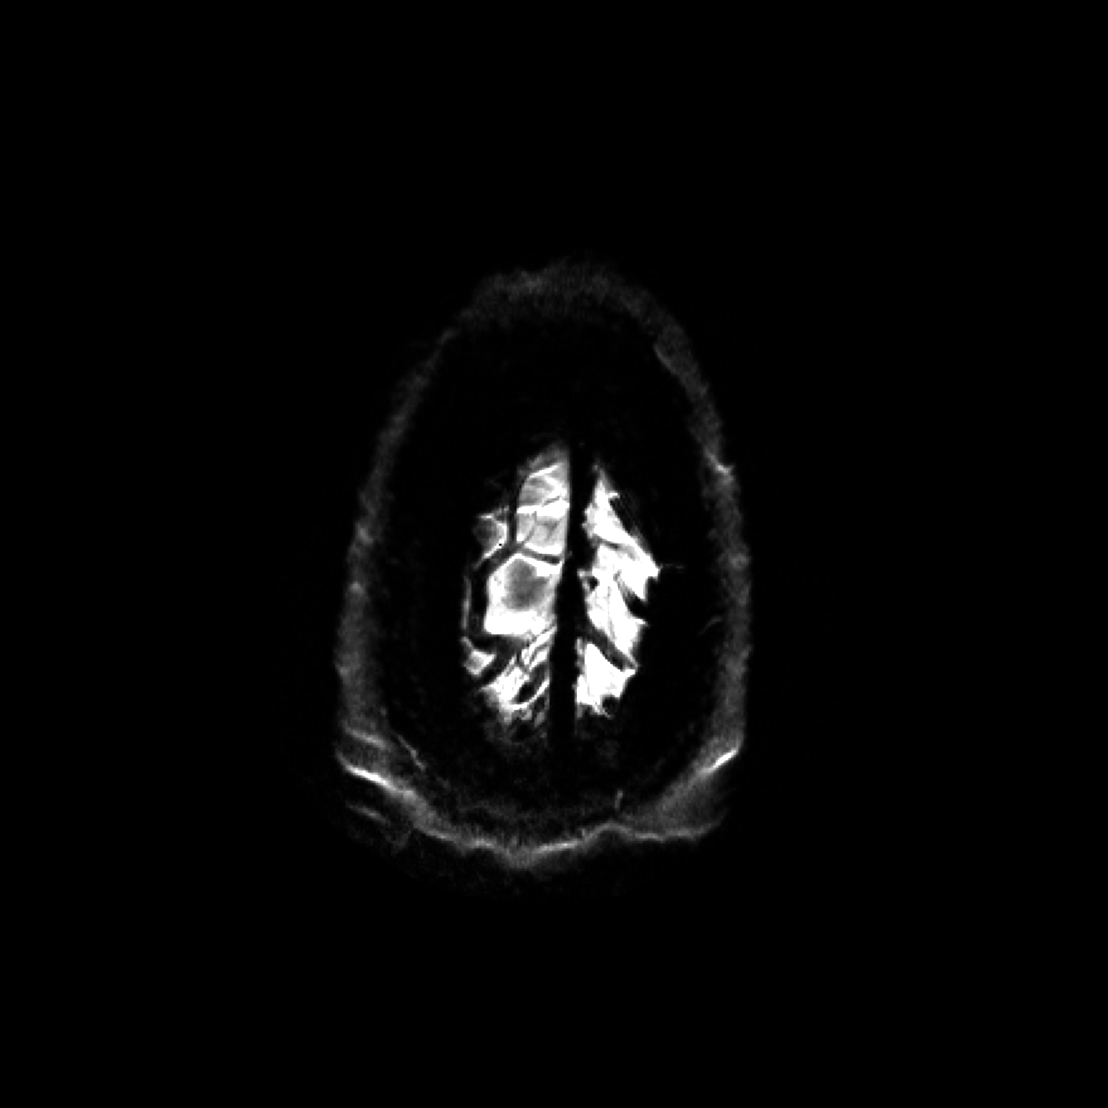
\includegraphics[width=.10\textwidth]{figures/DWI_dir-0_slice-1.png}};

		\node[inner sep=0pt] (DWI-slice1-dir3) at (.30, -1.70)
		{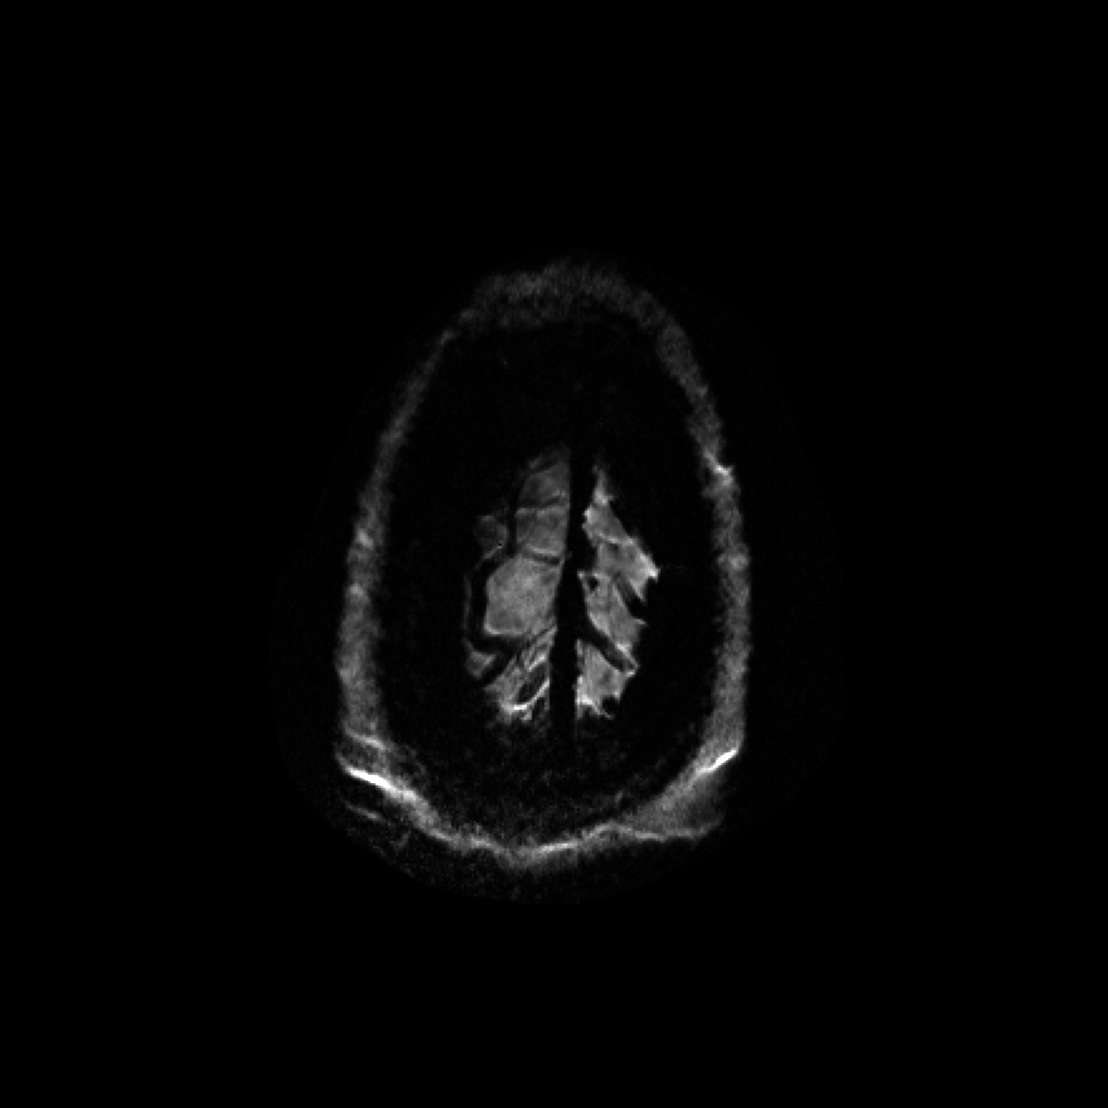
\includegraphics[width=.10\textwidth]{figures/DWI_dir-3_slice-1.png}};

		\node[inner sep=0pt] (DWI-slice1-dir2) at (.15, -1.85)
		{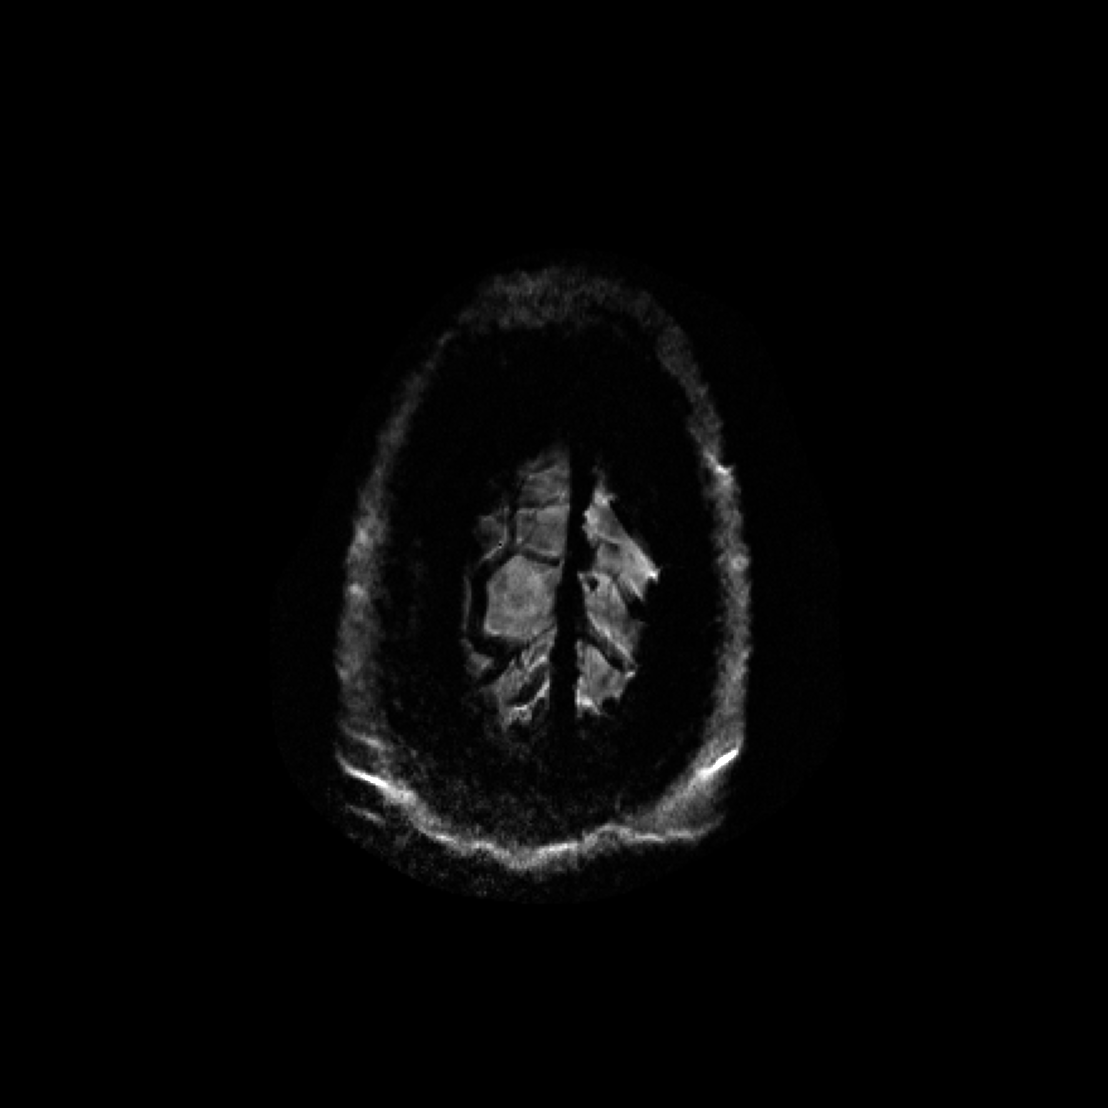
\includegraphics[width=.10\textwidth]{figures/DWI_dir-2_slice-1.png}};

		\node[inner sep=0pt] (DWI-slice1-dir1) at (0,-2.0)
		{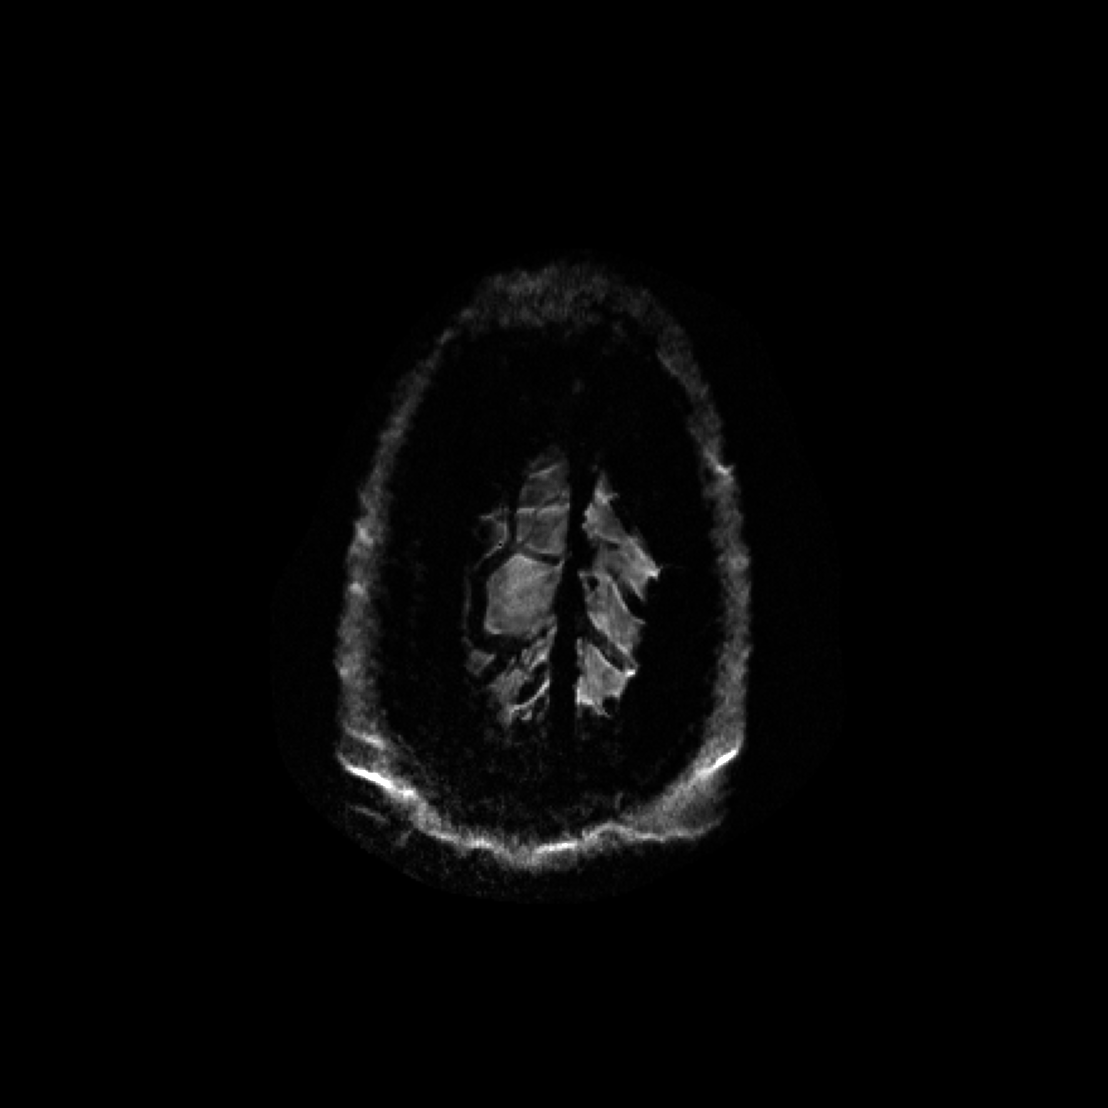
\includegraphics[width=.10\textwidth]{figures/DWI_dir-1_slice-1.png}};


		% Connection
		\draw[->, line width=0.5pt] (1.1, 0.25) -- (2.3, 0.25);
		\node[font=\tiny] at (1.65, 0.40) {\textbf{Multiply}};


		\node[font=\tiny] at (4.60, 1.6) {Shot Phase};
		\node[font=\tiny] at (4.55, 1.3) {[$x$,~$y$,~$z$,~$q$,~$s$]};

		% Shots - slice0
		\node[inner sep=0pt] (Shot0-slice0-dir0) at (3.45,.45)
		{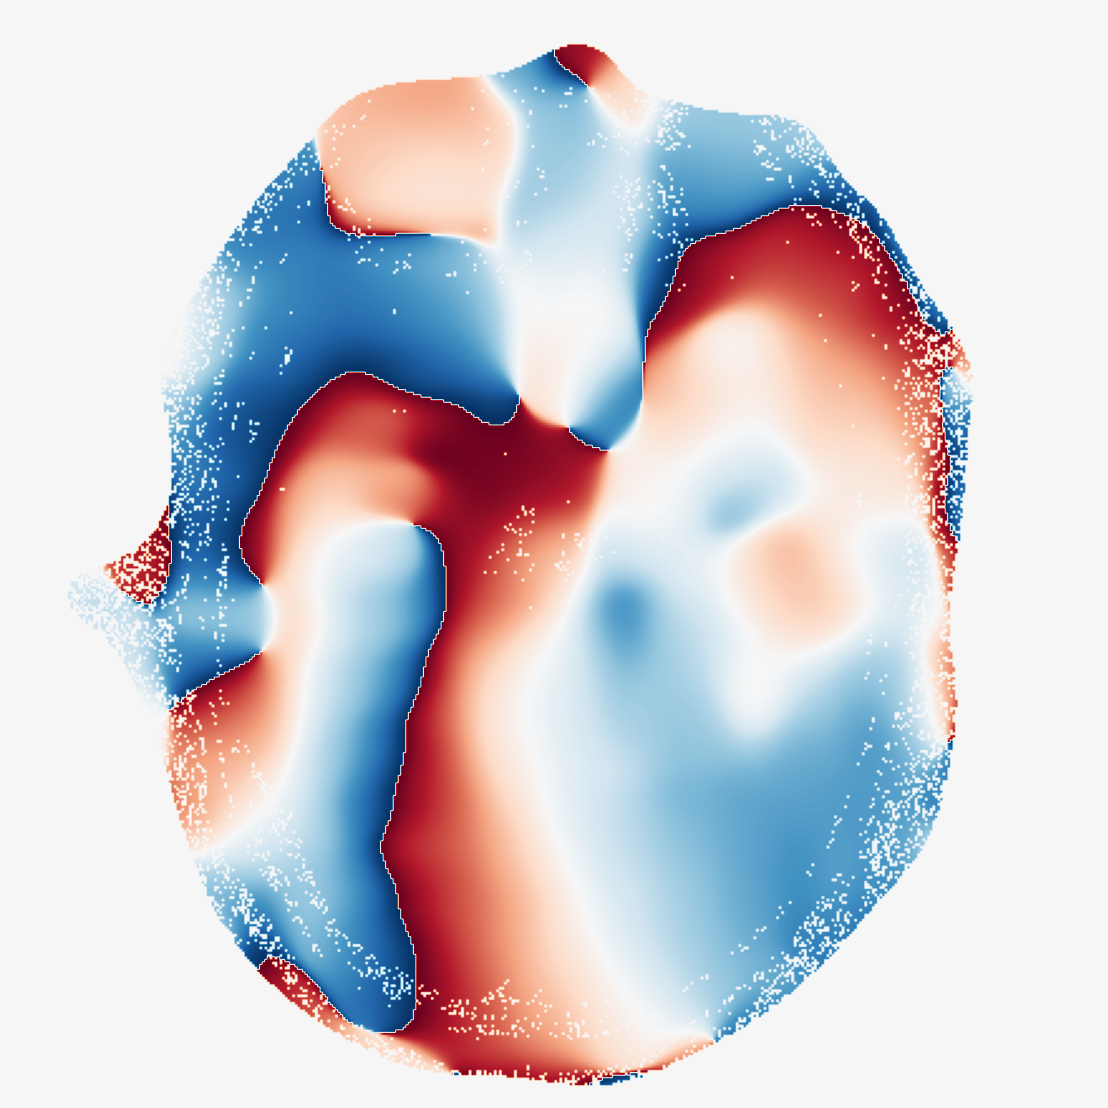
\includegraphics[width=.10\textwidth]{figures/DWI_dir-0_slice-0_shot-0.png}};
		\node[inner sep=0pt] (Shot0-slice0-dir3) at (3.30,.30)
		{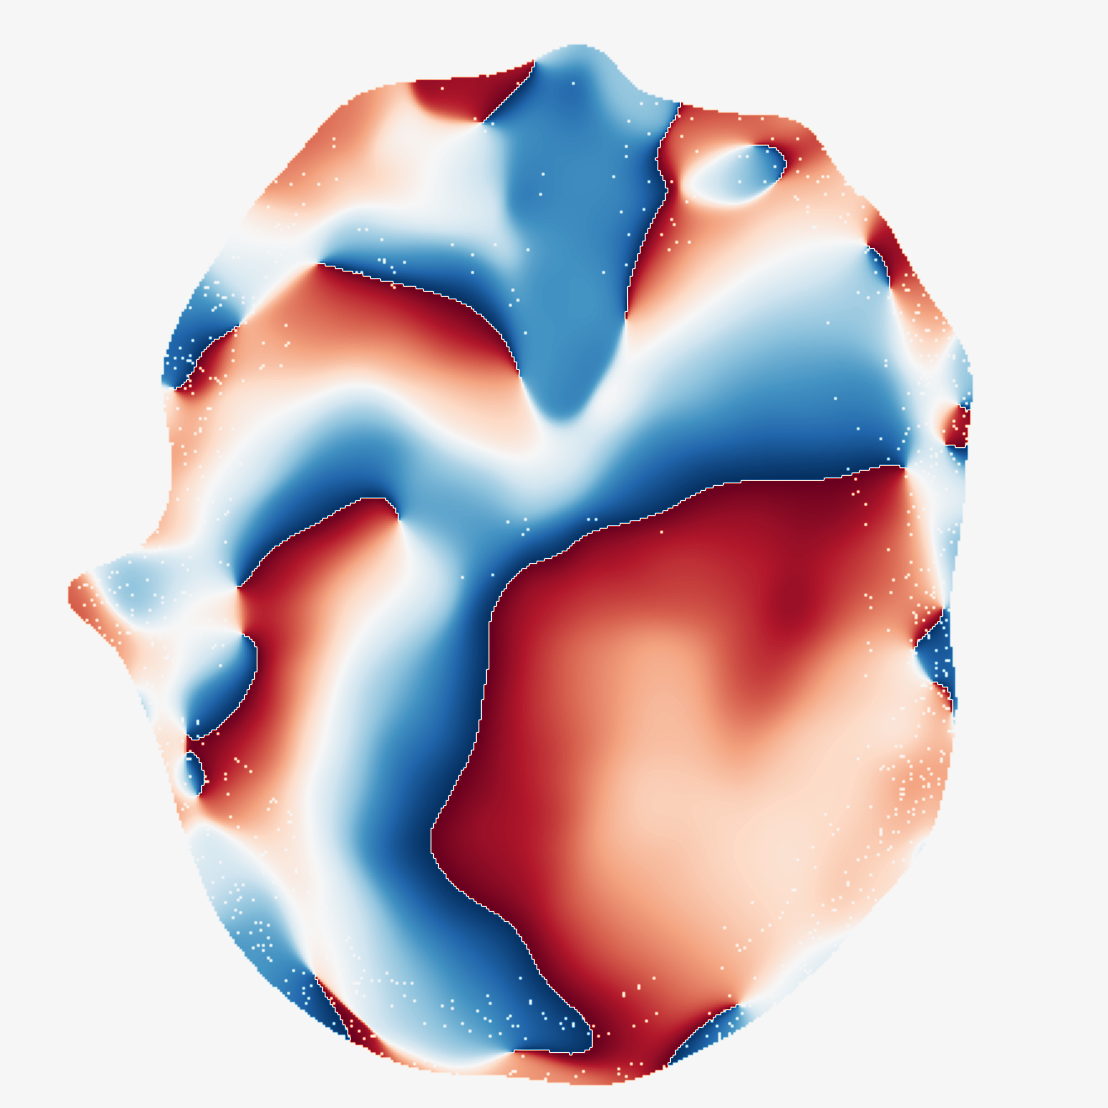
\includegraphics[width=.10\textwidth]{figures/DWI_dir-3_slice-0_shot-0.png}};
		\node[inner sep=0pt] (Shot0-slice0-dir2) at (3.15,.15)
		{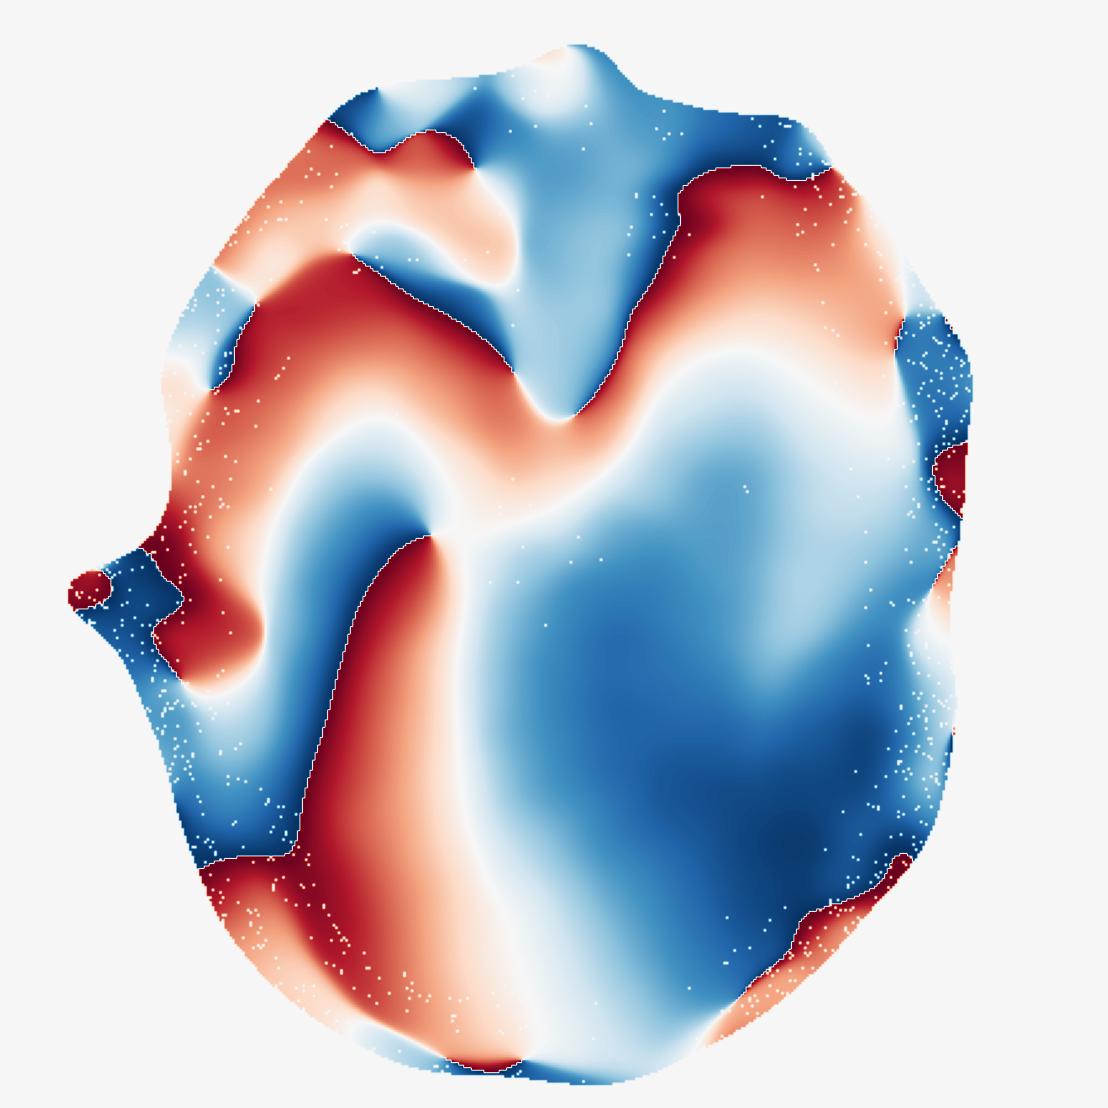
\includegraphics[width=.10\textwidth]{figures/DWI_dir-2_slice-0_shot-0.png}};
		\node[inner sep=0pt] (Shot0-slice0-dir1) at (3.00,.00)
		{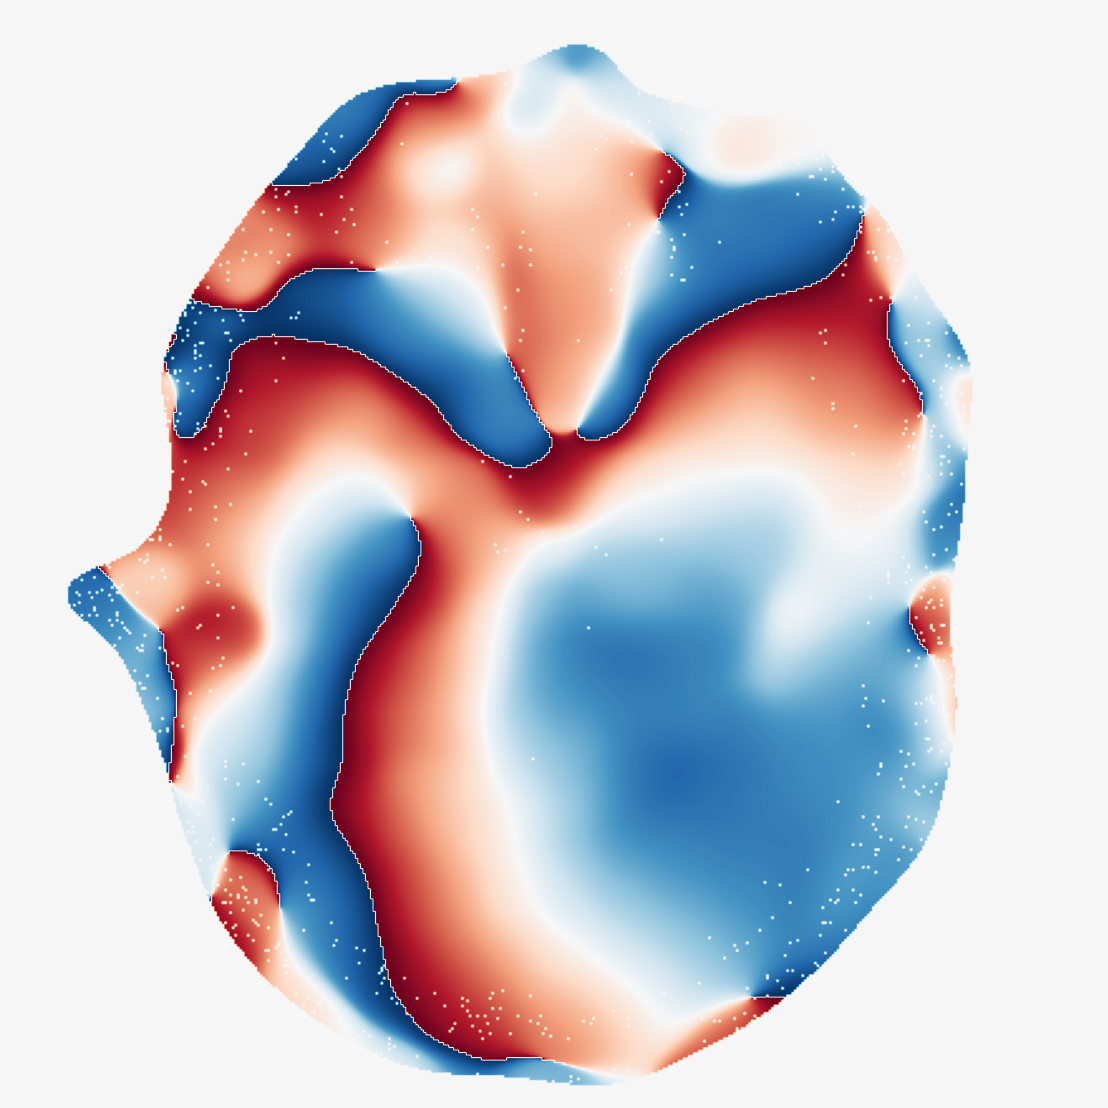
\includegraphics[width=.10\textwidth]{figures/DWI_dir-1_slice-0_shot-0.png}};

		\fill (4.2, 0.2) circle (1pt);
		\fill (4.3, 0.2) circle (1pt);
		\fill (4.4, 0.2) circle (1pt);

		\node[inner sep=0pt] (Shot4-slice0-dir0) at (5.65,.45)
		{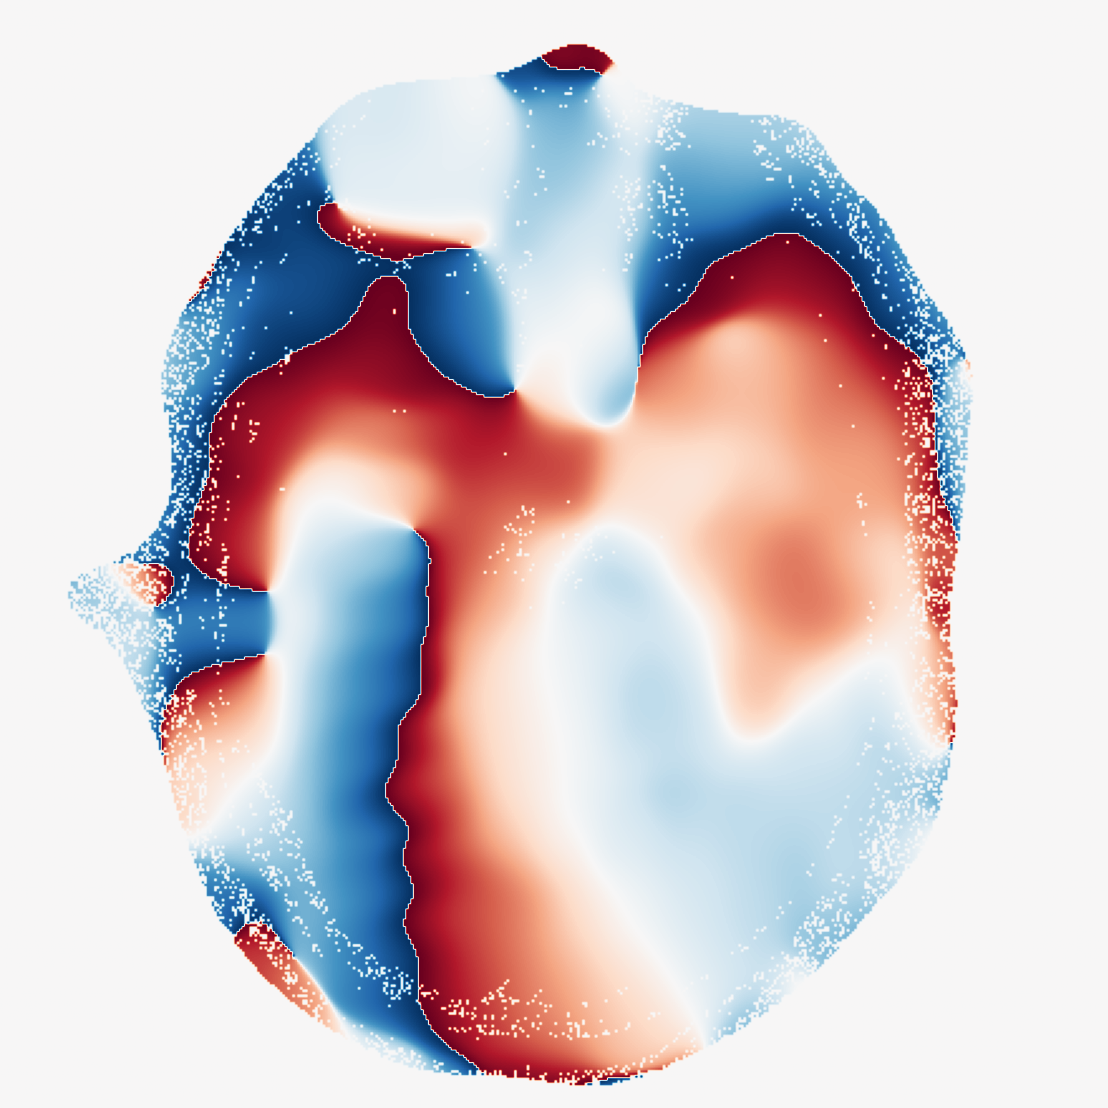
\includegraphics[width=.10\textwidth]{figures/DWI_dir-0_slice-0_shot-4.png}};
		\node[inner sep=0pt] (Shot4-slice0-dir3) at (5.50,.30)
		{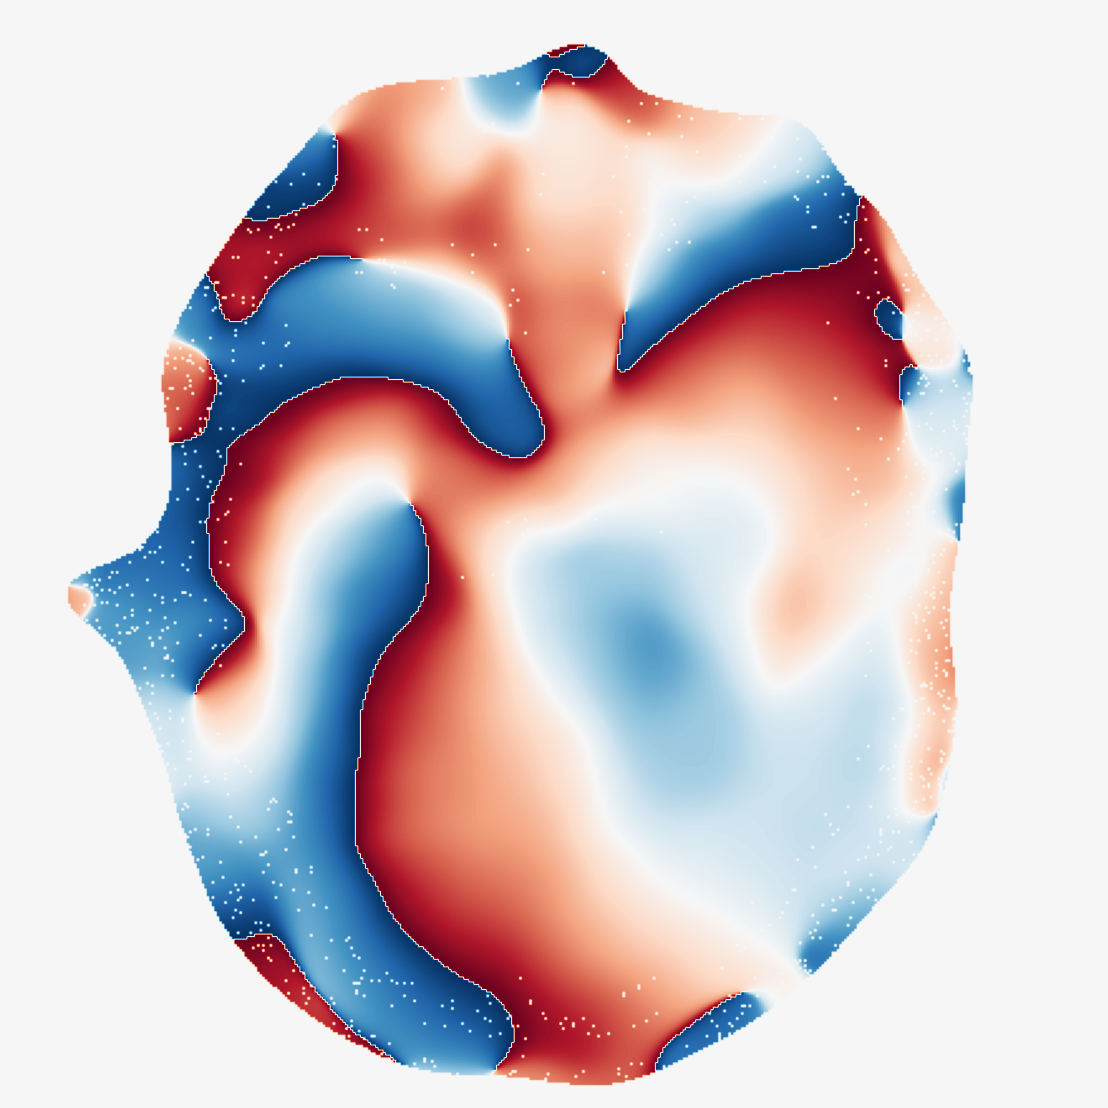
\includegraphics[width=.10\textwidth]{figures/DWI_dir-3_slice-0_shot-4.png}};
		\node[inner sep=0pt] (Shot4-slice0-dir2) at (5.35,.15)
		{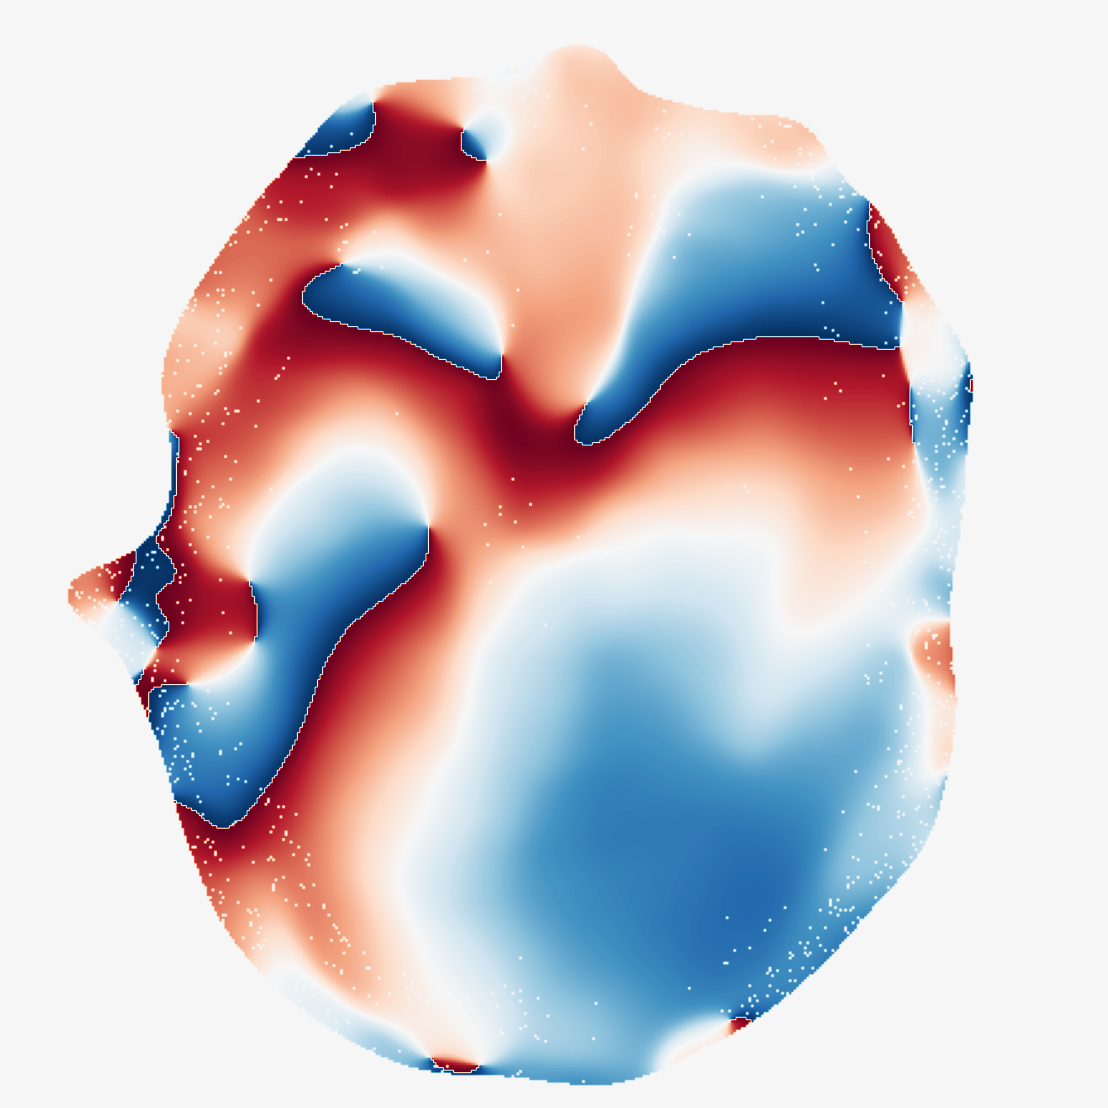
\includegraphics[width=.10\textwidth]{figures/DWI_dir-2_slice-0_shot-4.png}};
		\node[inner sep=0pt] (Shot4-slice0-dir1) at (5.20,.00)
		{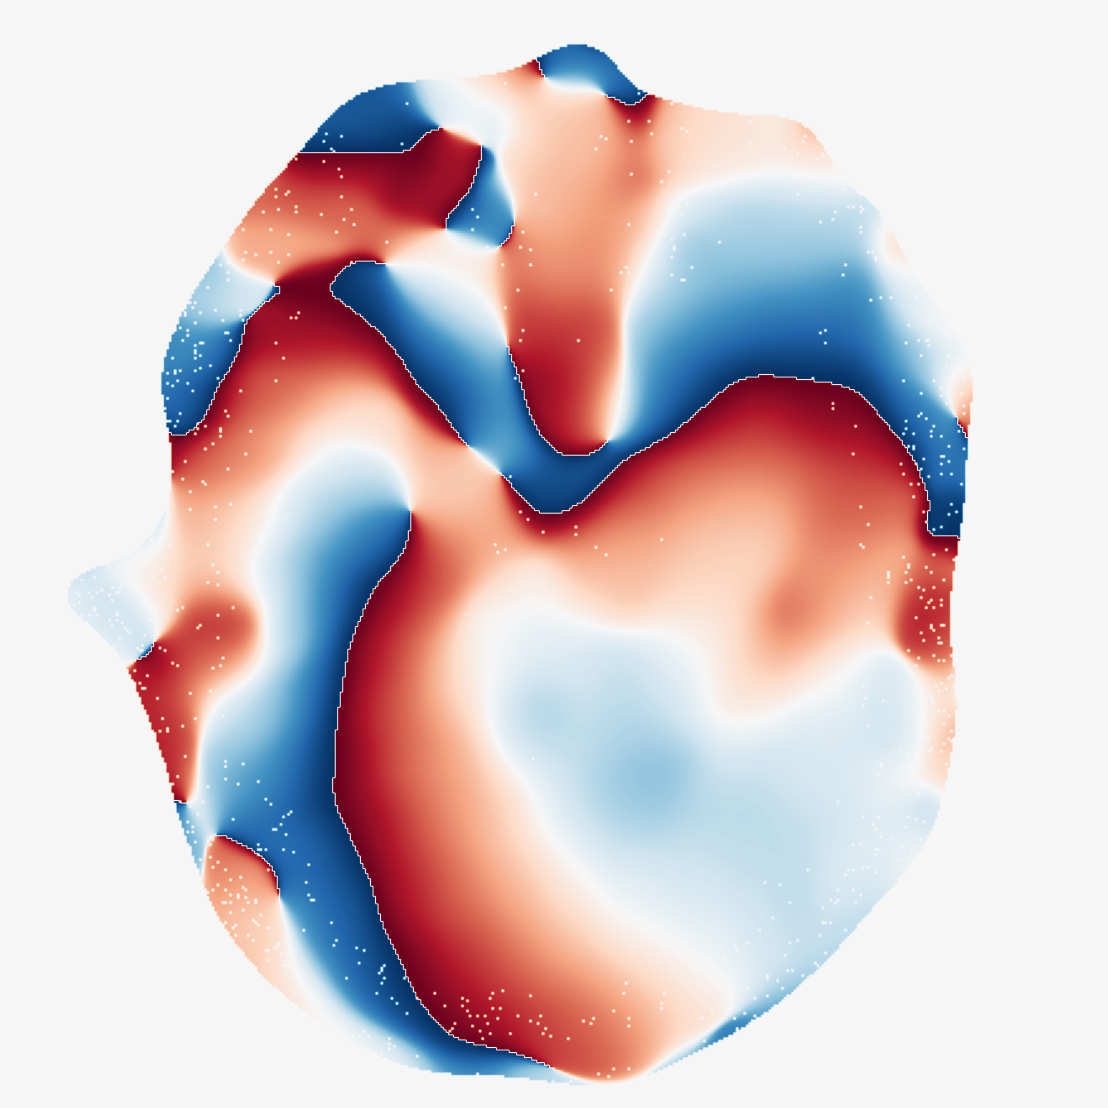
\includegraphics[width=.10\textwidth]{figures/DWI_dir-1_slice-0_shot-4.png}};

		\draw[->, line width=0.5pt] (4, -0.5) -- (4.2, -0.5);
		\node[font=\tiny] at (4.3, -0.5) {$s$};


		% Shots - slice1
		\node[inner sep=0pt] (Shot0-slice1-dir0) at (3.45,-1.55)
		{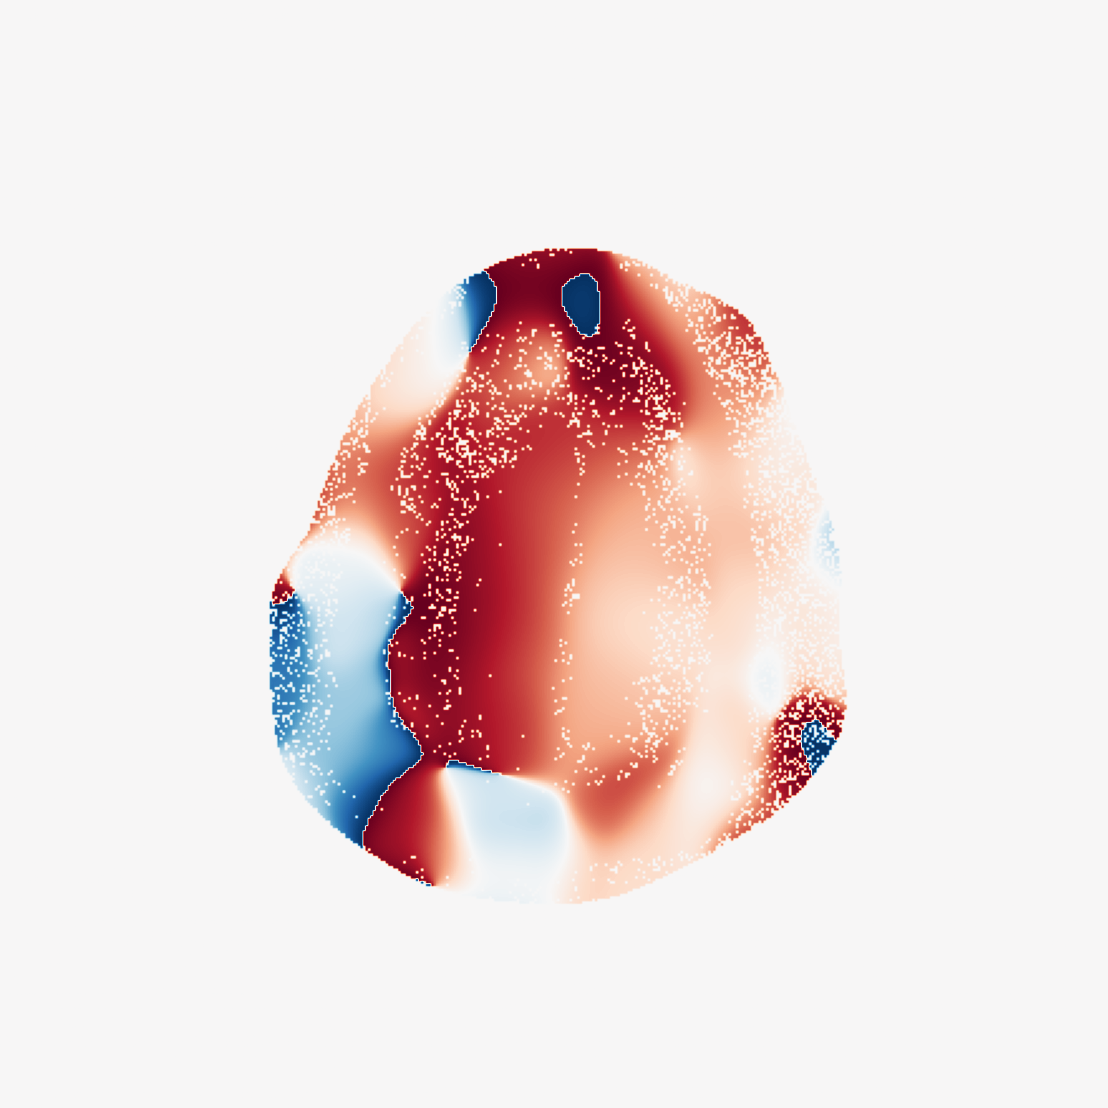
\includegraphics[width=.10\textwidth]{figures/DWI_dir-0_slice-1_shot-0.png}};
		\node[inner sep=0pt] (Shot0-slice1-dir3) at (3.30,-1.70)
		{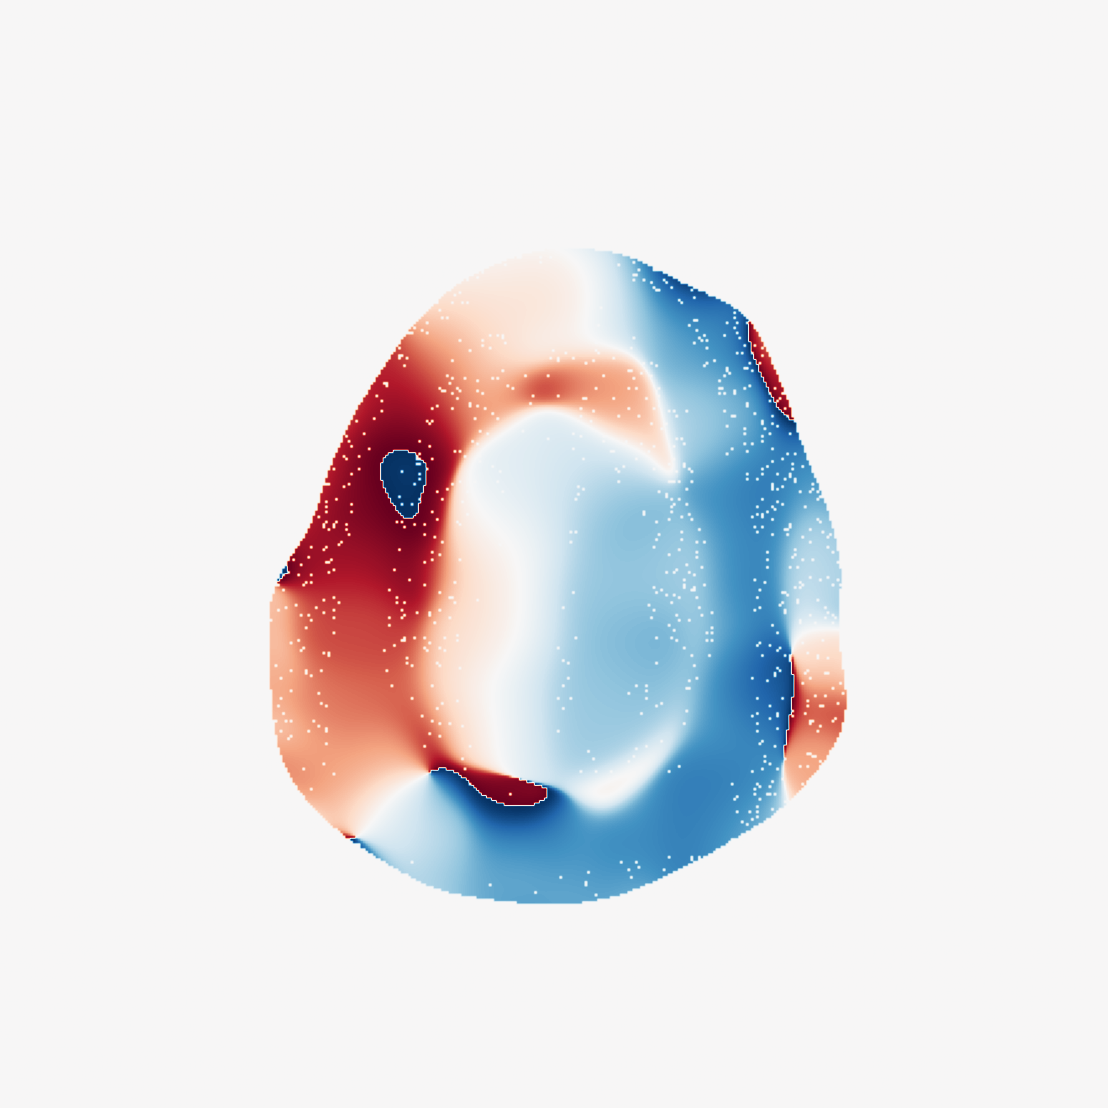
\includegraphics[width=.10\textwidth]{figures/DWI_dir-3_slice-1_shot-0.png}};
		\node[inner sep=0pt] (Shot0-slice1-dir2) at (3.15,-1.85)
		{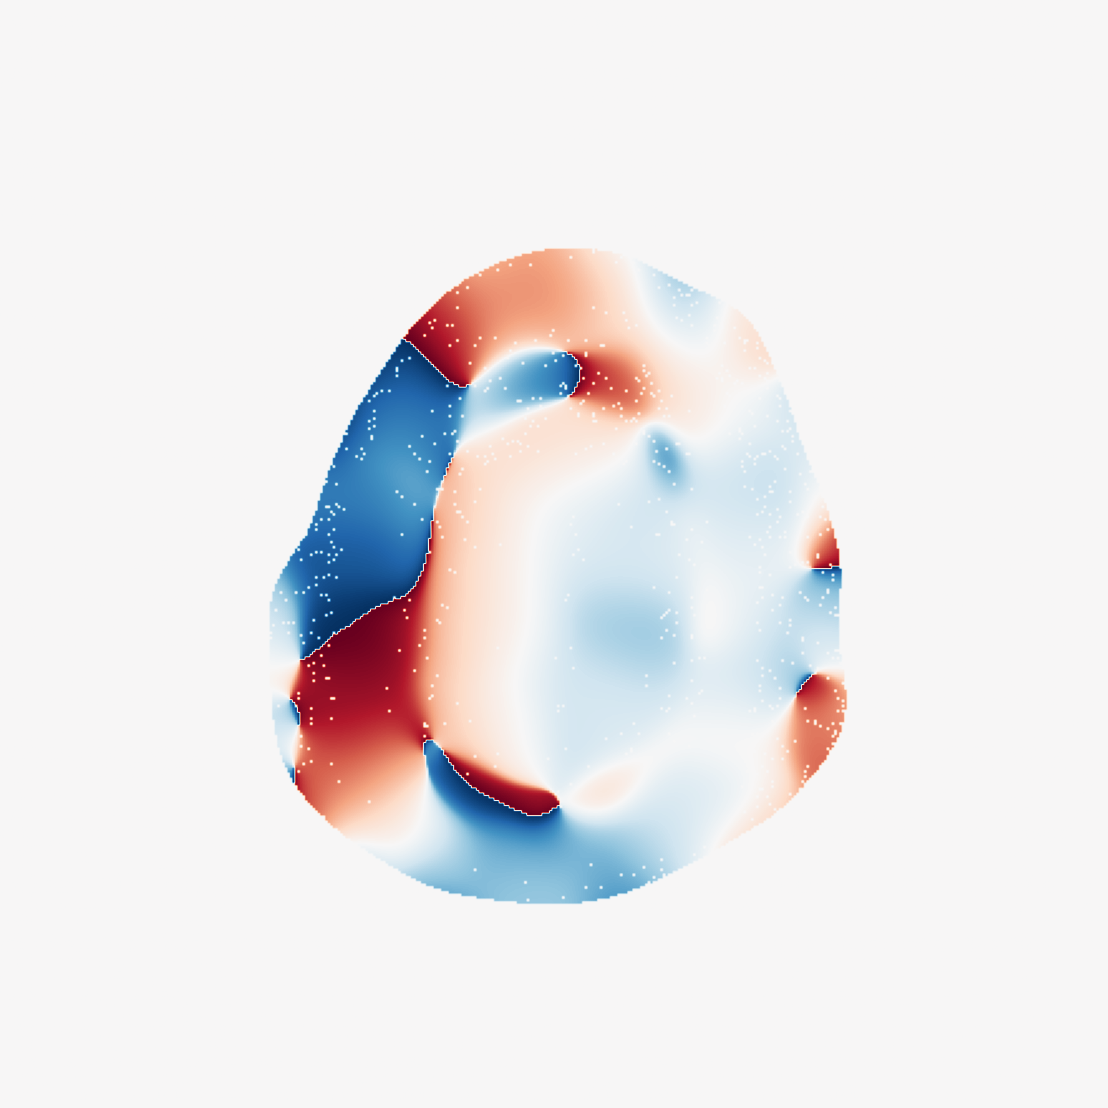
\includegraphics[width=.10\textwidth]{figures/DWI_dir-2_slice-1_shot-0.png}};
		\node[inner sep=0pt] (Shot0-slice1-dir1) at (3.00,-2.00)
		{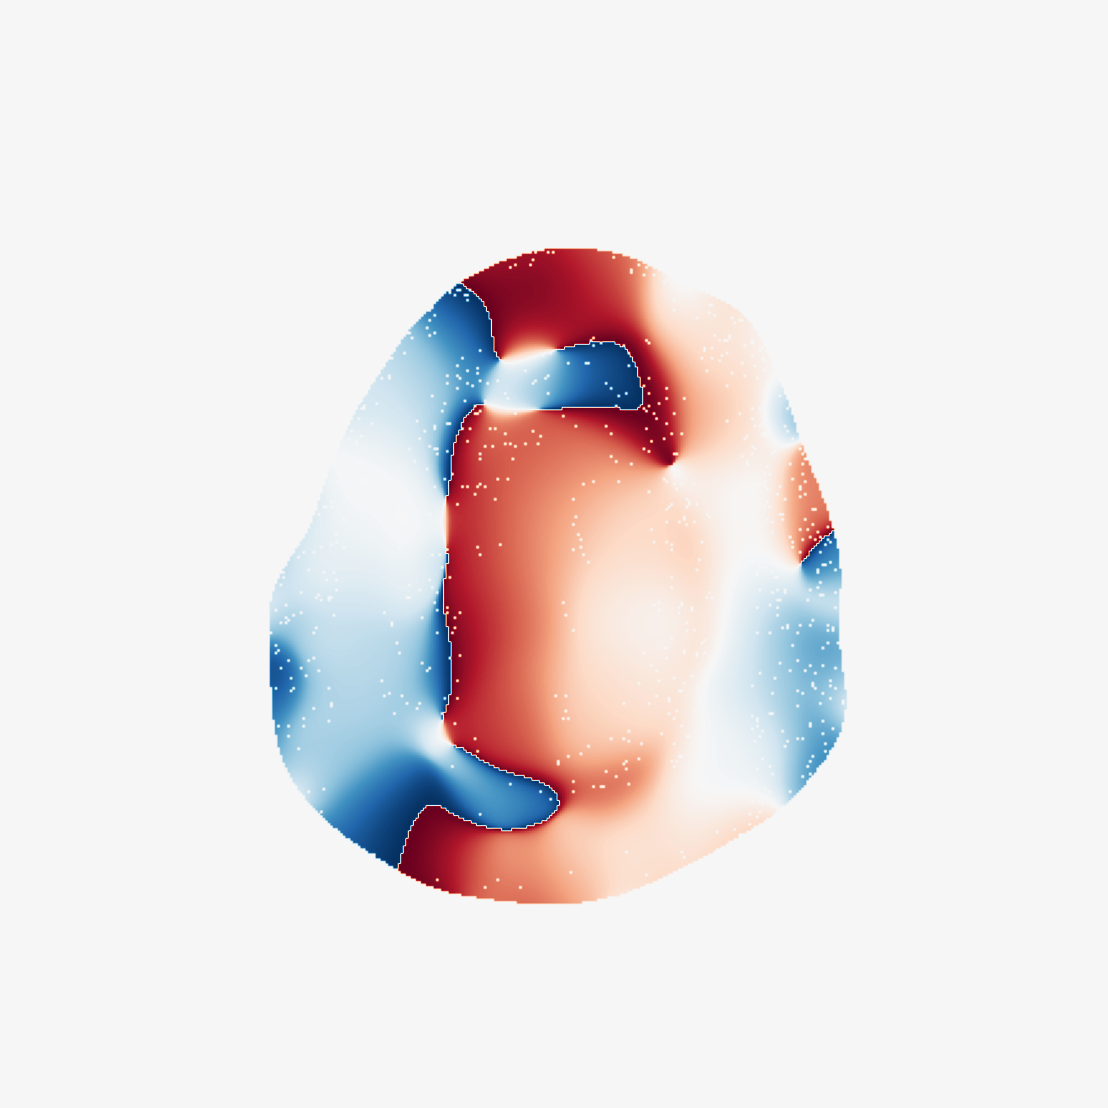
\includegraphics[width=.10\textwidth]{figures/DWI_dir-1_slice-1_shot-0.png}};

		\fill (4.2, -1.8) circle (1pt);
		\fill (4.3, -1.8) circle (1pt);
		\fill (4.4, -1.8) circle (1pt);

		\node[inner sep=0pt] (Shot4-slice1-dir0) at (5.65,-1.55)
		{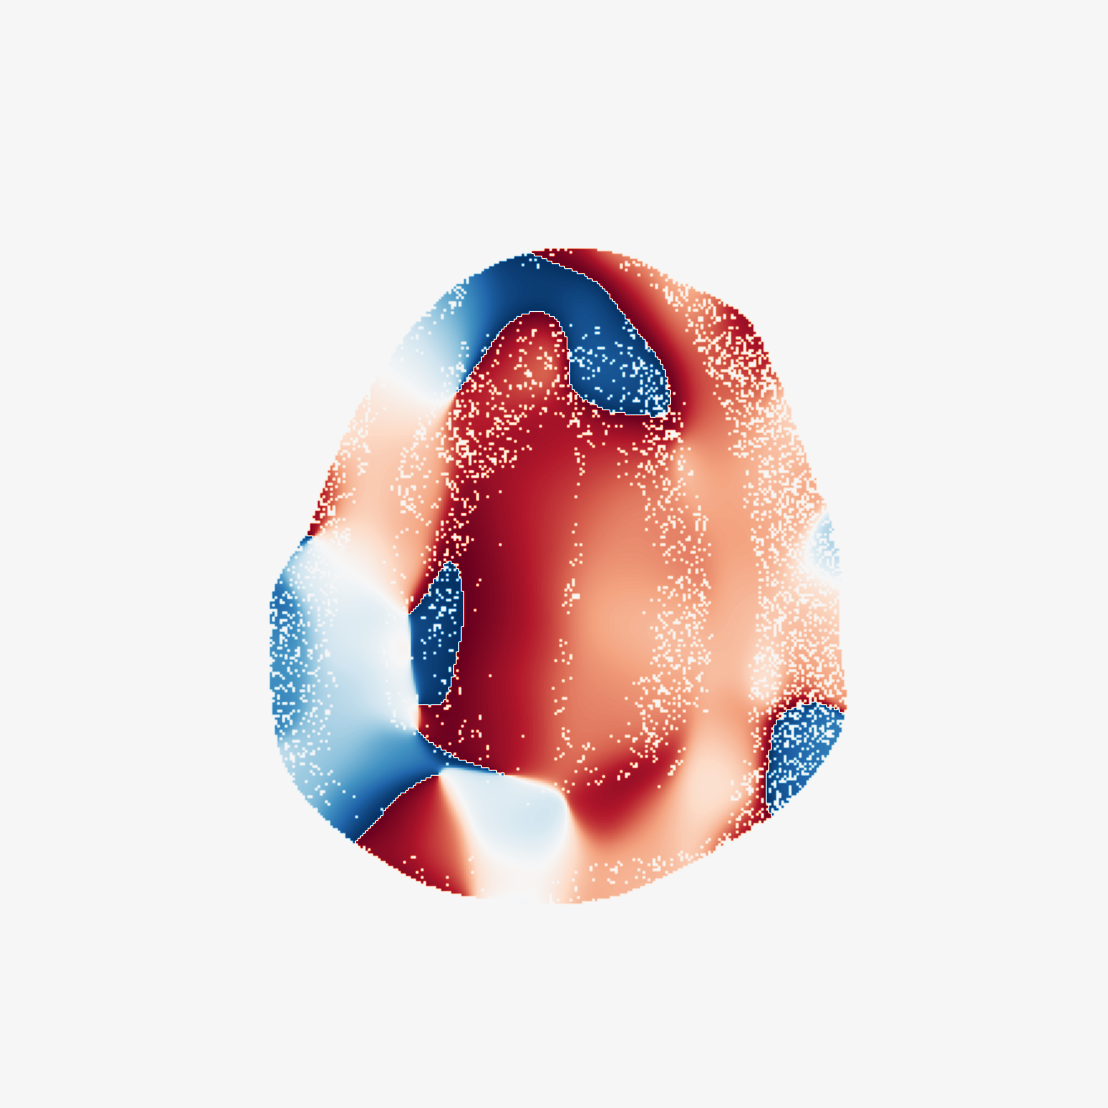
\includegraphics[width=.10\textwidth]{figures/DWI_dir-0_slice-1_shot-4.png}};
		\node[inner sep=0pt] (Shot4-slice1-dir3) at (5.50,-1.70)
		{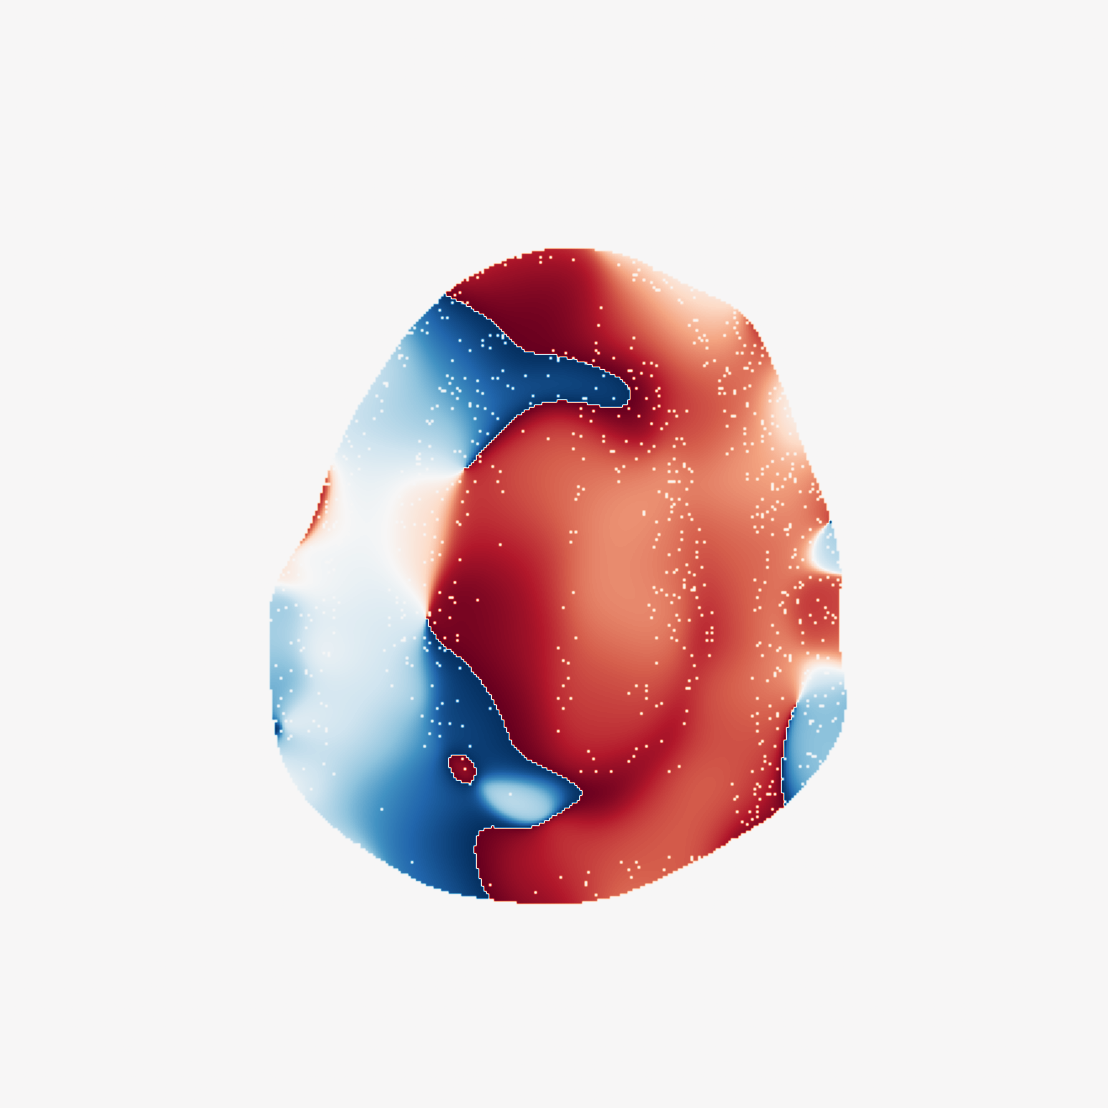
\includegraphics[width=.10\textwidth]{figures/DWI_dir-3_slice-1_shot-4.png}};
		\node[inner sep=0pt] (Shot4-slice1-dir2) at (5.35,-1.85)
		{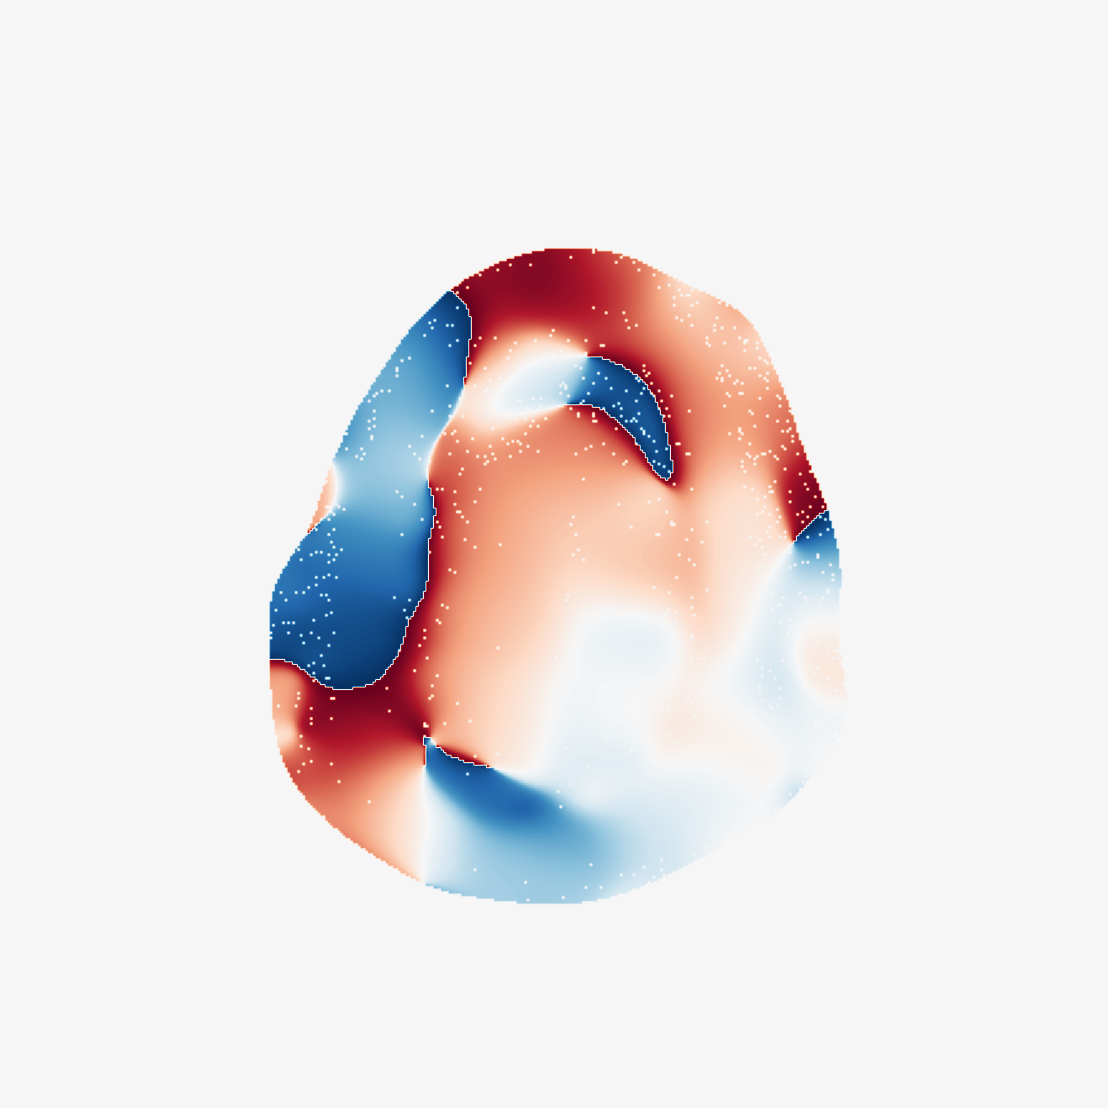
\includegraphics[width=.10\textwidth]{figures/DWI_dir-2_slice-1_shot-4.png}};
		\node[inner sep=0pt] (Shot4-slice1-dir1) at (5.20,-2.00)
		{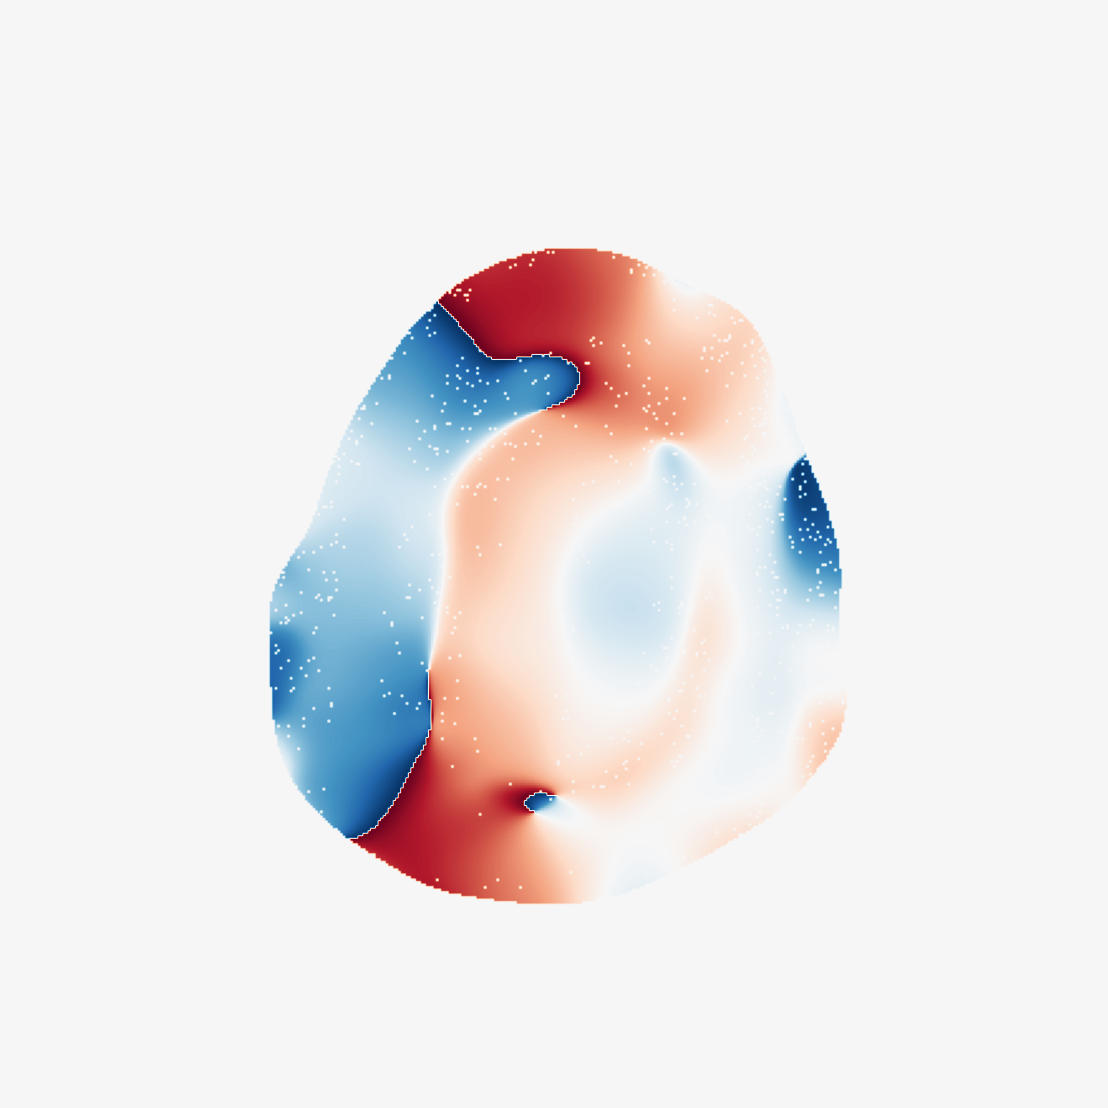
\includegraphics[width=.10\textwidth]{figures/DWI_dir-1_slice-1_shot-4.png}};

		\draw[->, line width=0.5pt] (1.1, -1.75) -- (2.3, -1.75);

		\draw[- , line width=0.5pt] (6.3,  0.2) -- (6.5,  0.2);
		\draw[- , line width=0.5pt] (6.3, -1.8) -- (6.5, -1.8);
		\draw[- , line width=0.5pt] (6.5, -1.8) -- (6.5,  0.2);
		\draw[->, line width=0.5pt] (6.5, -0.75) -- (7, -0.75);

		% coils
		\draw[draw=black, line width=1pt] (7, -1) rectangle (7.5, -0.5);
		\node[font=\small] at (7.25, -0.75) {$\mathbf{S}$};

		\draw[->, line width=0.5pt] (7.5, -0.75) -- (8, -0.75);

		% FFT
		\draw[draw=black, line width=1pt] (8, -1) rectangle (8.5, -0.5);
		\node[font=\small] at (8.25, -0.75) {$\mathbf{F}$};

		\draw[->, line width=0.5pt] (8.5, -0.75) -- (9, -0.75);


		\node[font=\tiny] at (8.2, -1.8) {$\mathbf{S}$: Multiply with coil sensitivity maps};
		\node[font=\tiny] at (7.6, -2.1) {$\mathbf{F}$: Fourier transform};
		\node[font=\tiny] at (8.1, -2.4) {$\mathbf{P}$: Multiply with sampling pattern};

		% SMS
		\draw[draw=black, line width=1pt] (9, -1) rectangle (9.5, -0.5);
		\node[font=\small] at (9.25, -0.75) {$\mathbf{\Theta}$};
		\node[font=\tiny] at (9.7, -0.1) {Slice Phase \& Sum};

		\draw[->, line width=0.5pt] (9.5, -0.75) -- (10, -0.75);

		\draw[draw=black, line width=1pt] (10, -1) rectangle (10.5, -0.5);
		\node[font=\small] at (10.25, -0.75) {$\mathbf{\Sigma}$};

		\draw[->, line width=0.5pt] (10.5, -0.75) -- (11, -0.75);

		\draw[draw=red!60, line width=1pt, dotted, rounded corners=5pt] (8.75, -1.25) rectangle (10.75, 0.25);

		\node[font=\tiny] at (9.75, 1.6) {Multi Band (MB)};
		\node[font=\tiny] at (9.75, 1.3) {[$x$,~$y$,~$1$,~$c$,~$q$,~$s$]};

		% mask
		\draw[draw=black, line width=1pt] (11, -1) rectangle (11.5, -0.5);
		\node[font=\small] at (11.25, -0.75) {$\mathbf{P}$};

		\draw[->, line width=0.5pt] (11.5, -0.75) -- (11.9, -0.75);

		% k-space - coil0
		\node[inner sep=0pt] (ksp-Shot0-dir0) at (12.95,-1.55)
		{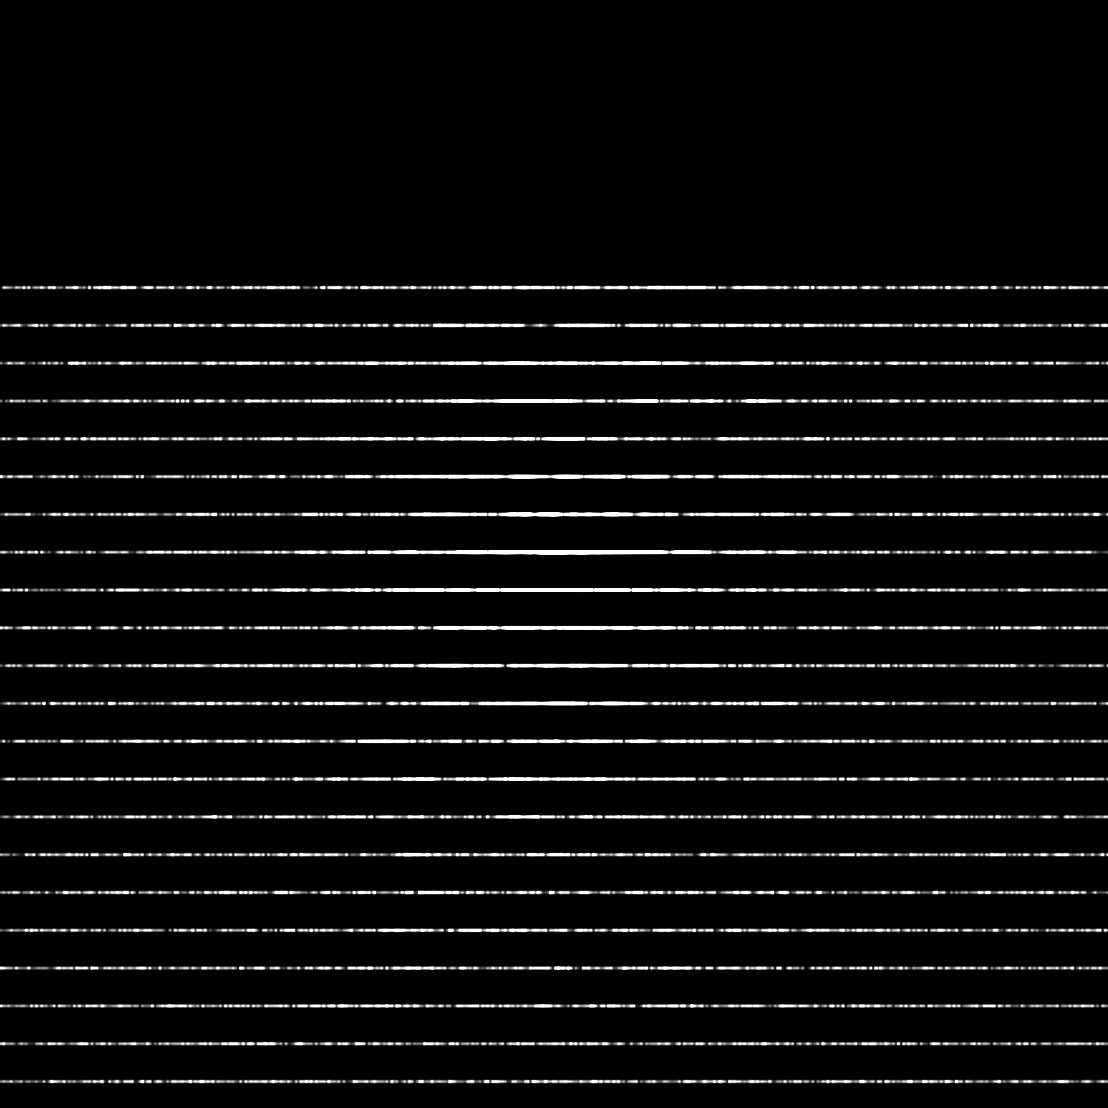
\includegraphics[width=.10\textwidth]{figures/ksp_dir-0_coil-0_shot-0.png}};
		\node[inner sep=0pt] (ksp-Shot0-dir3) at (12.80,-1.70)
		{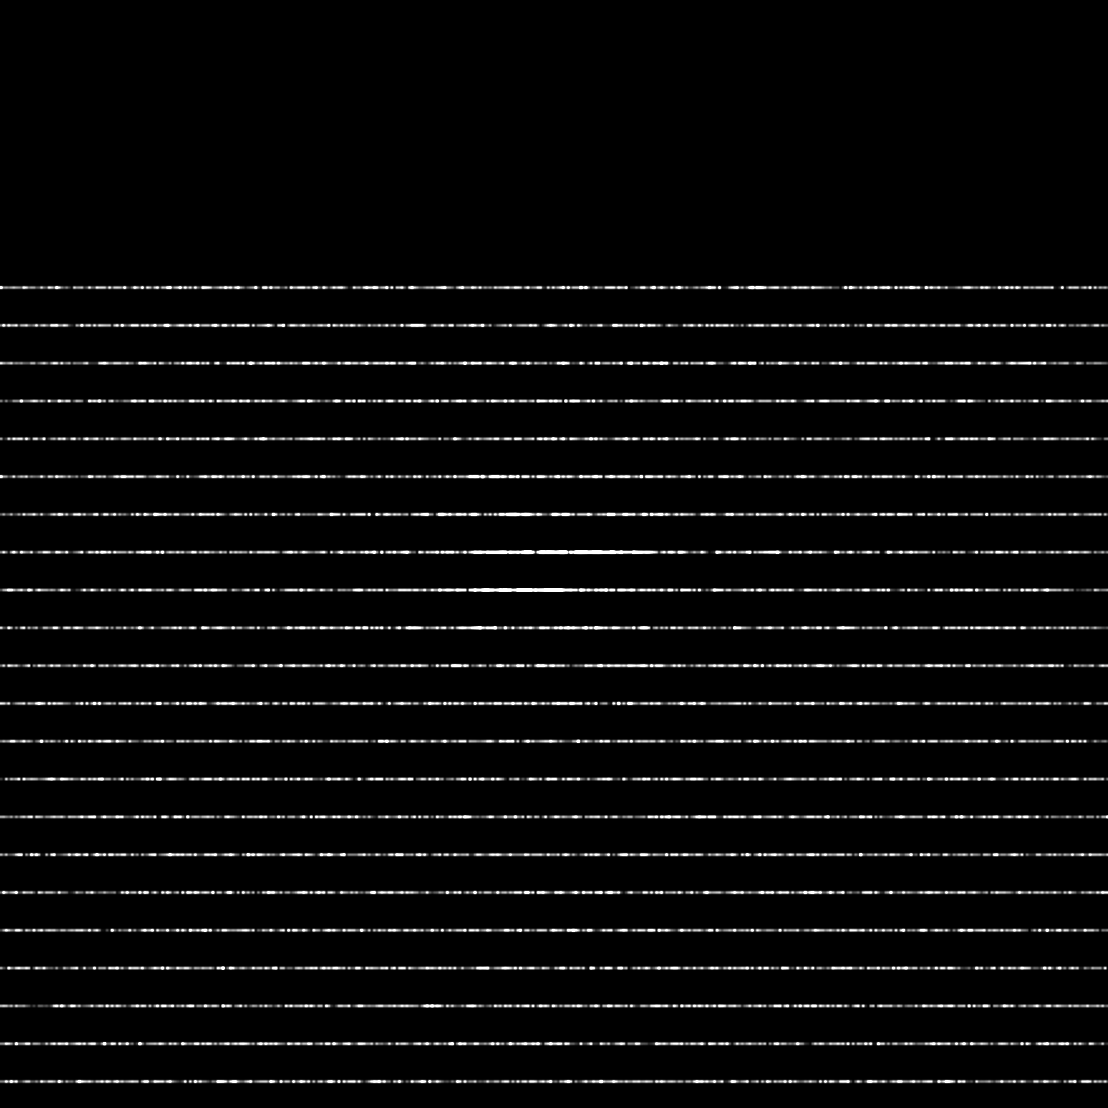
\includegraphics[width=.10\textwidth]{figures/ksp_dir-3_coil-0_shot-0.png}};
		\node[inner sep=0pt] (ksp-Shot0-dir2) at (12.65,-1.85)
		{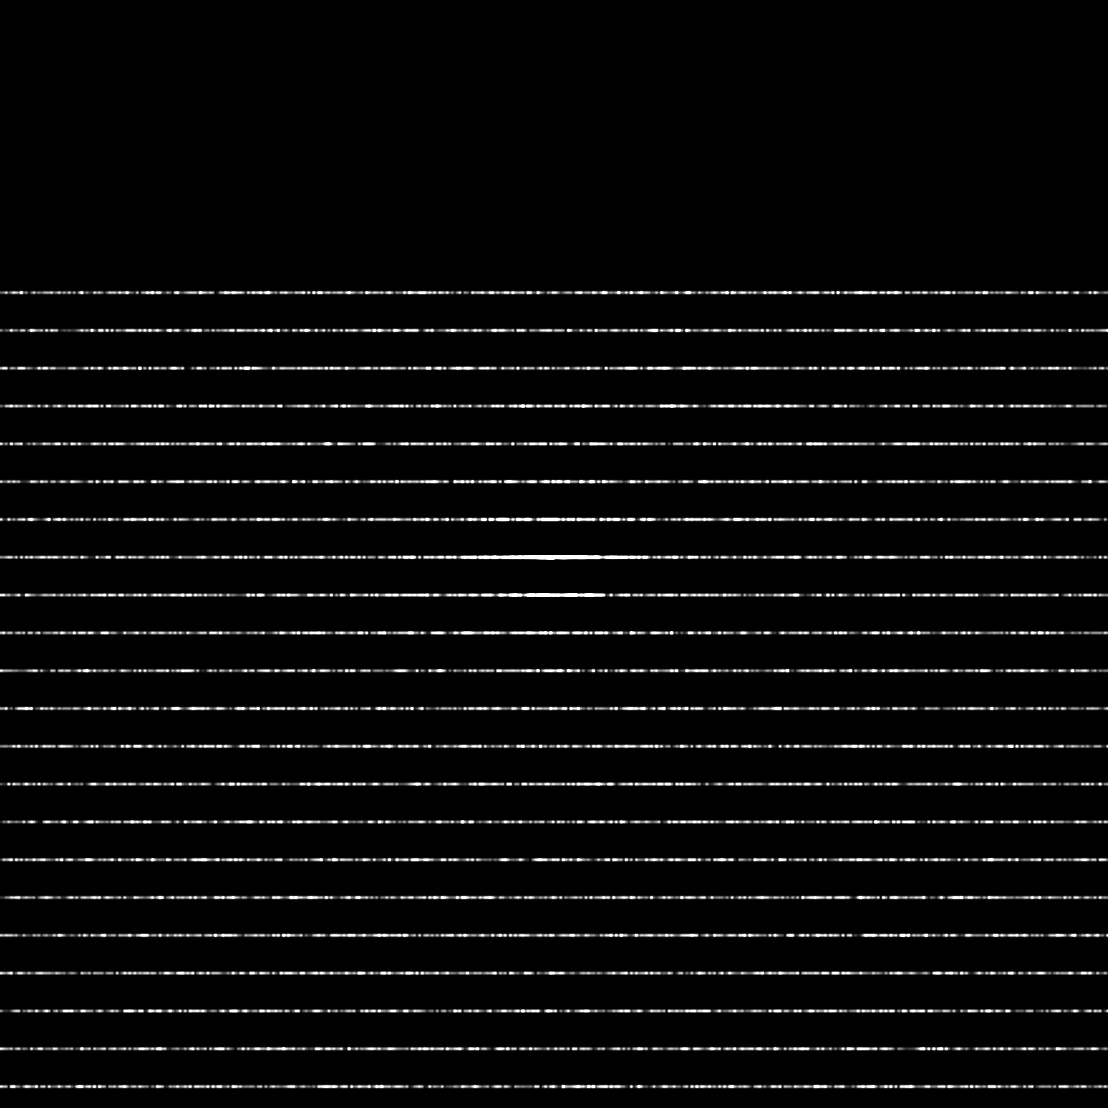
\includegraphics[width=.10\textwidth]{figures/ksp_dir-2_coil-0_shot-0.png}};
		\node[inner sep=0pt] (ksp-Shot0-dir1) at (12.50,-2.00)
		{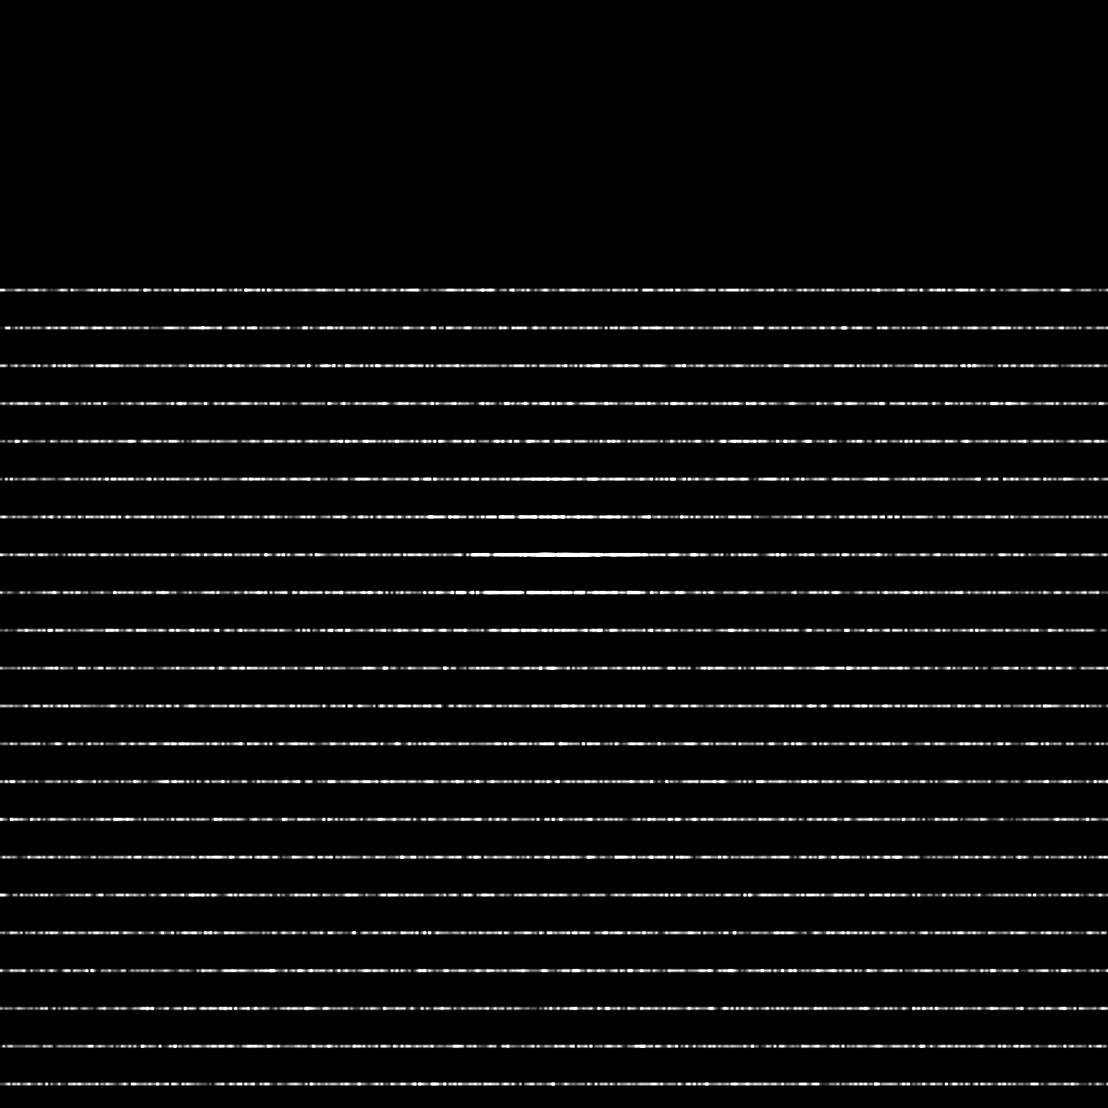
\includegraphics[width=.10\textwidth]{figures/ksp_dir-1_coil-0_shot-0.png}};

		\fill (13.7, -1.65) circle (1pt);
		\fill (13.8, -1.65) circle (1pt);
		\fill (13.9, -1.65) circle (1pt);

		\node[inner sep=0pt] (ksp-Shot4-dir0) at (15.15,-1.55)
		{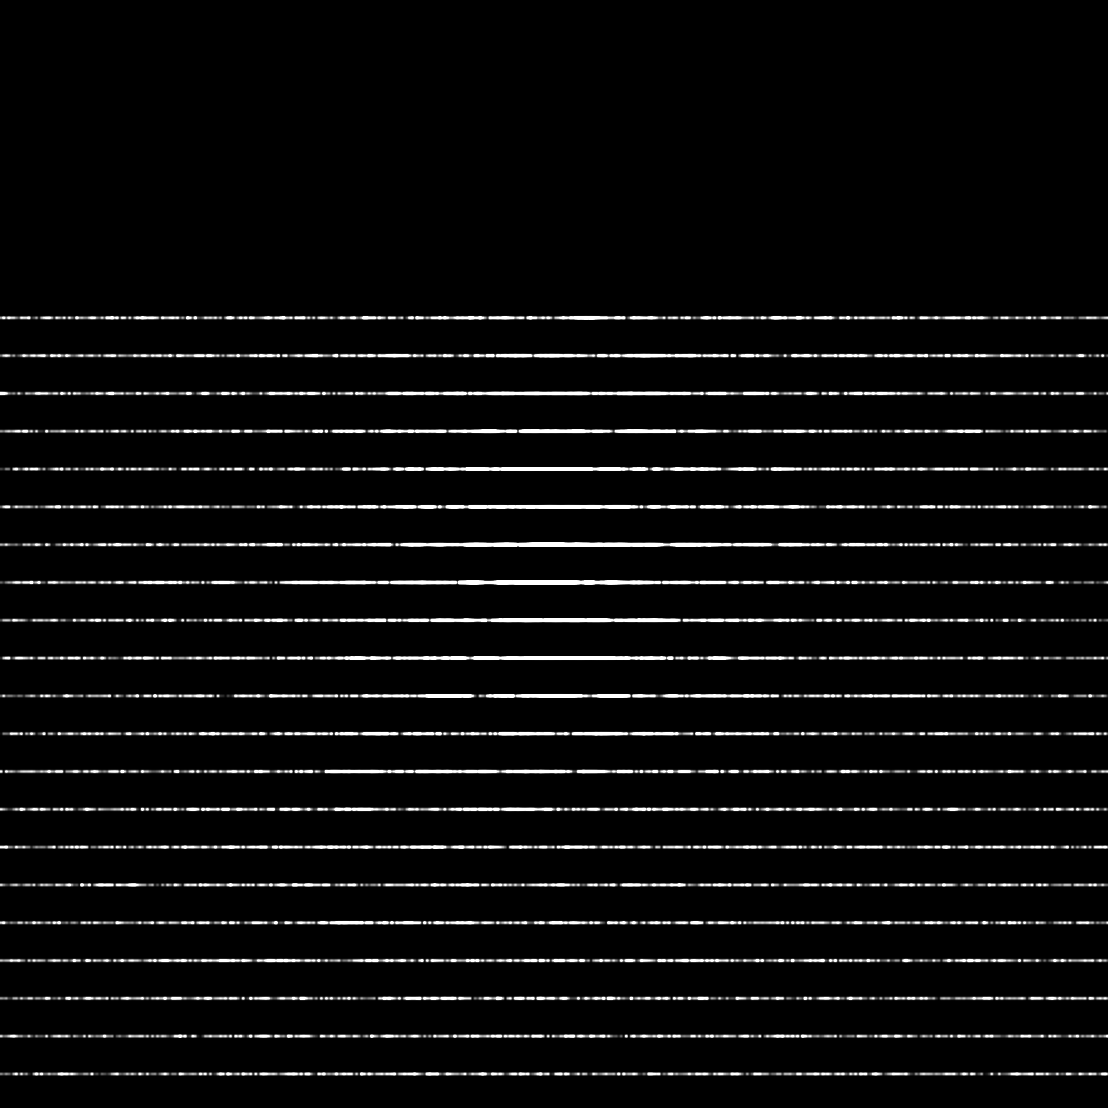
\includegraphics[width=.10\textwidth]{figures/ksp_dir-0_coil-0_shot-4.png}};
		\node[inner sep=0pt] (ksp-Shot4-dir3) at (15.00,-1.70)
		{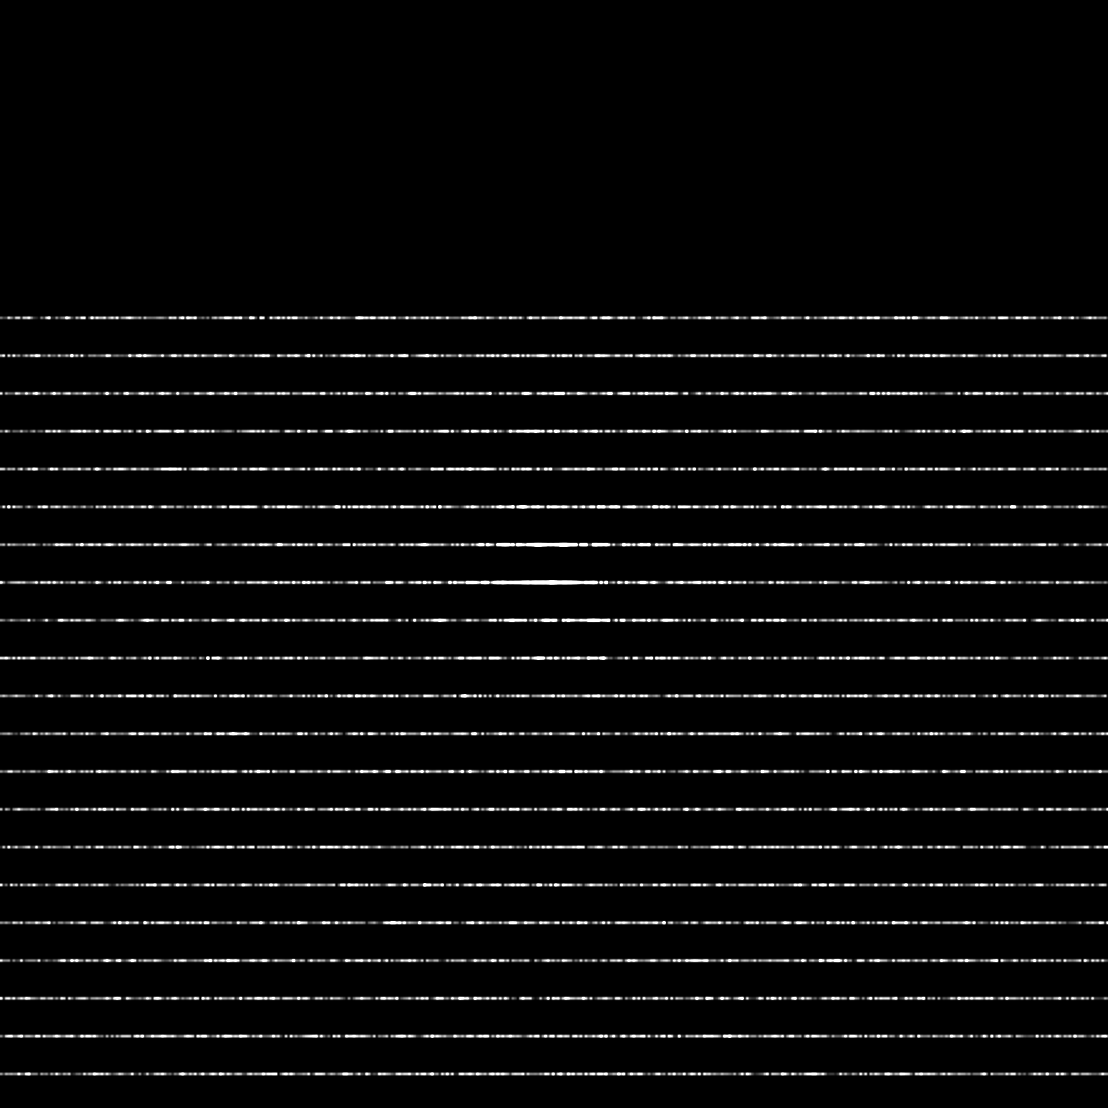
\includegraphics[width=.10\textwidth]{figures/ksp_dir-3_coil-0_shot-4.png}};
		\node[inner sep=0pt] (ksp-Shot4-dir2) at (14.85,-1.85)
		{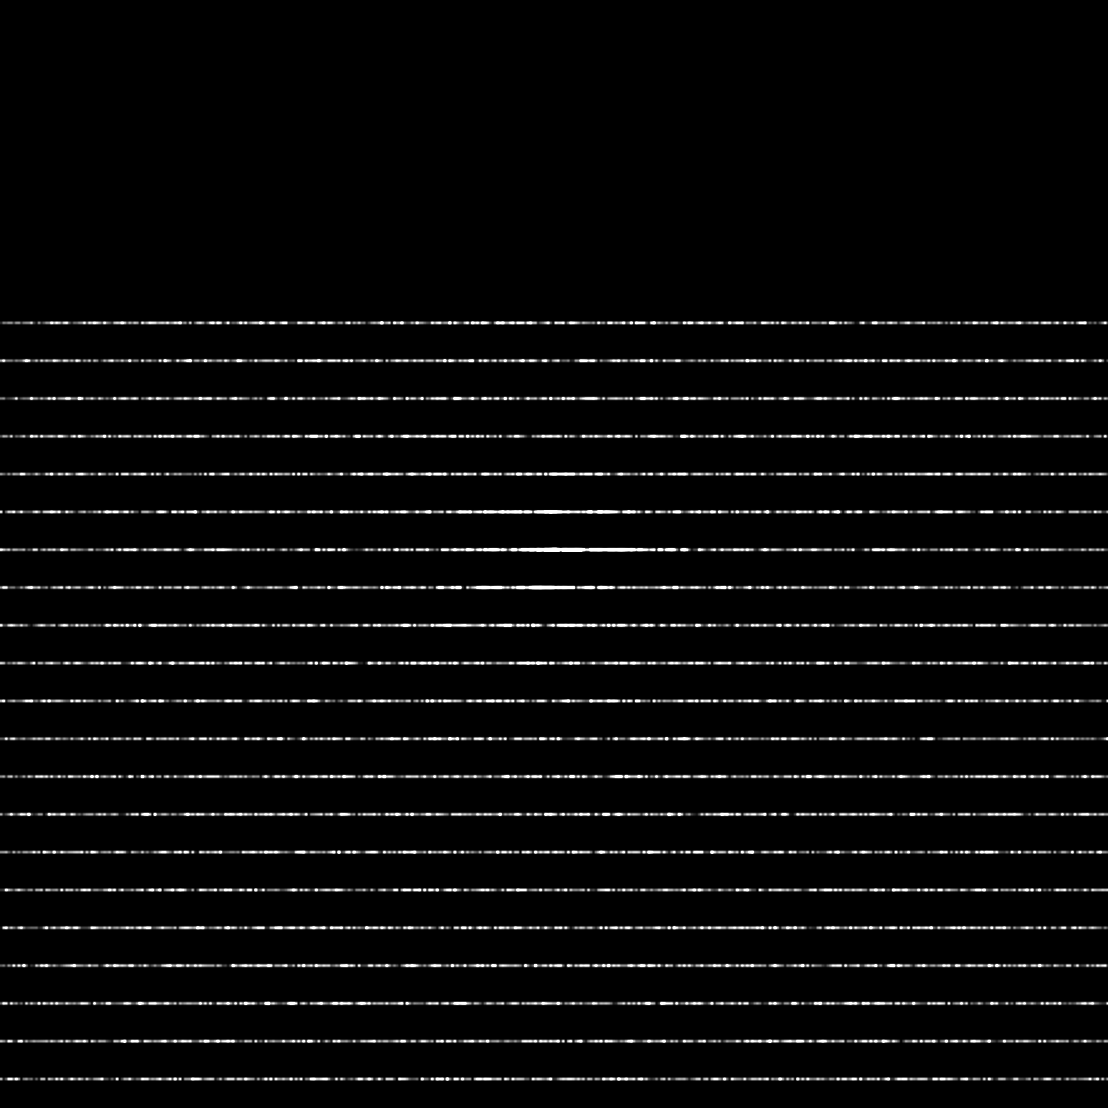
\includegraphics[width=.10\textwidth]{figures/ksp_dir-2_coil-0_shot-4.png}};
		\node[inner sep=0pt] (ksp-Shot4-dir1) at (14.70,-2.00)
		{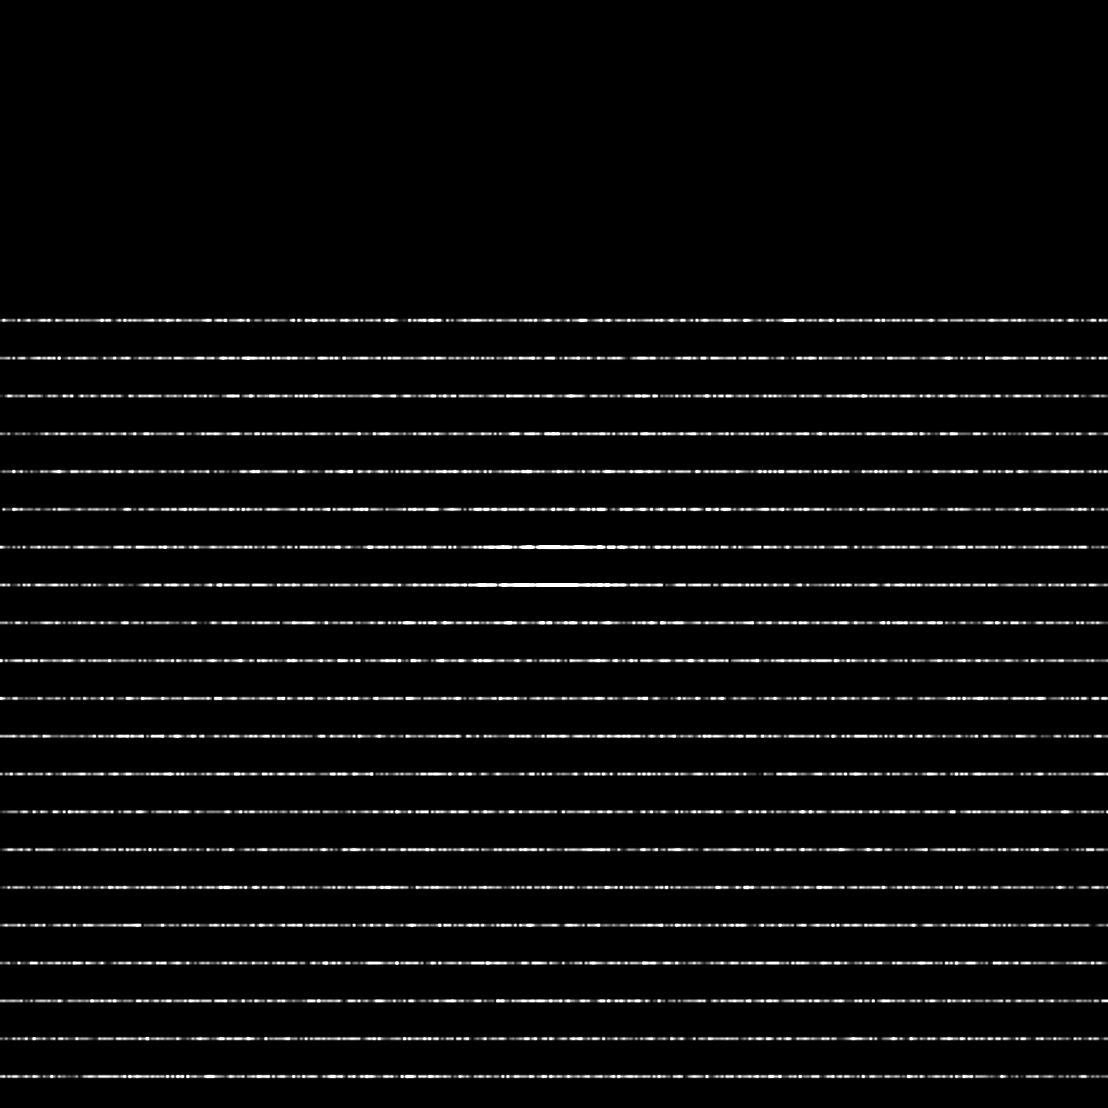
\includegraphics[width=.10\textwidth]{figures/ksp_dir-1_coil-0_shot-4.png}};

		% k-space - coil1
		\node[inner sep=0pt] (ksp-Shot0-dir0) at (12.95, 0.65)
		{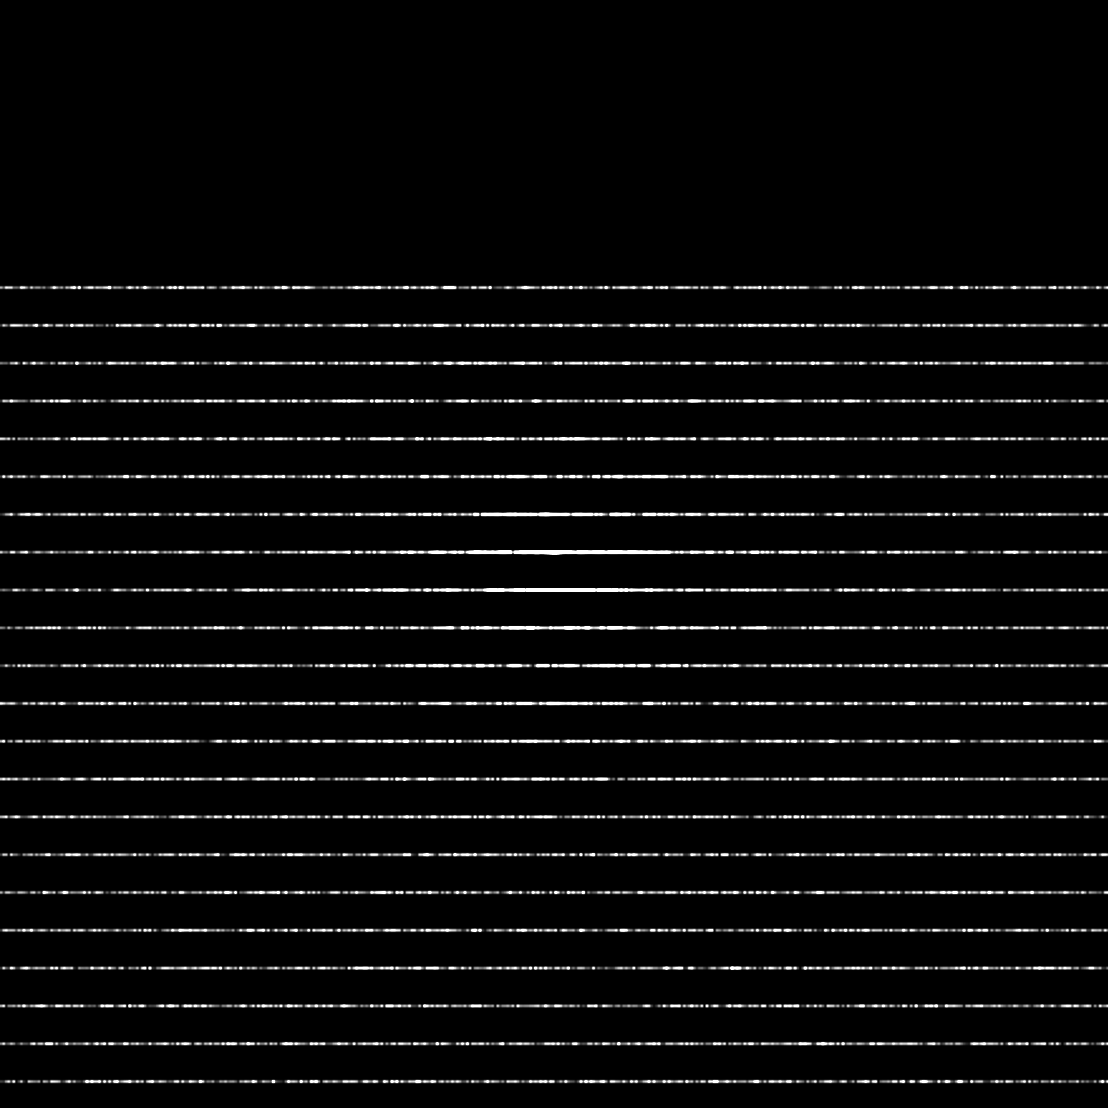
\includegraphics[width=.10\textwidth]{figures/ksp_dir-0_coil-1_shot-0.png}};
		\node[inner sep=0pt] (ksp-Shot0-dir3) at (12.80, 0.50)
		{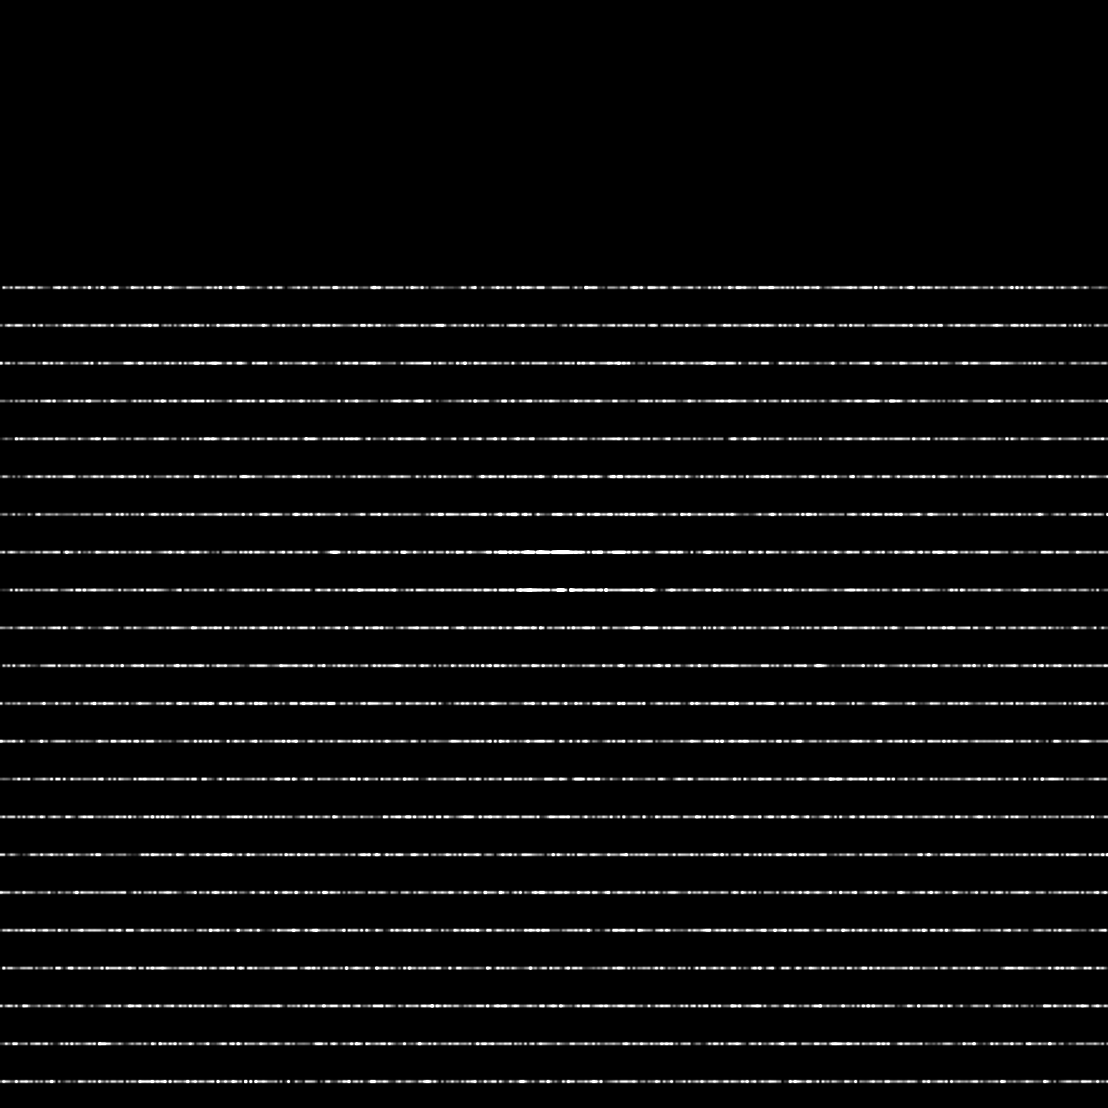
\includegraphics[width=.10\textwidth]{figures/ksp_dir-3_coil-1_shot-0.png}};
		\node[inner sep=0pt] (ksp-Shot0-dir2) at (12.65, 0.35)
		{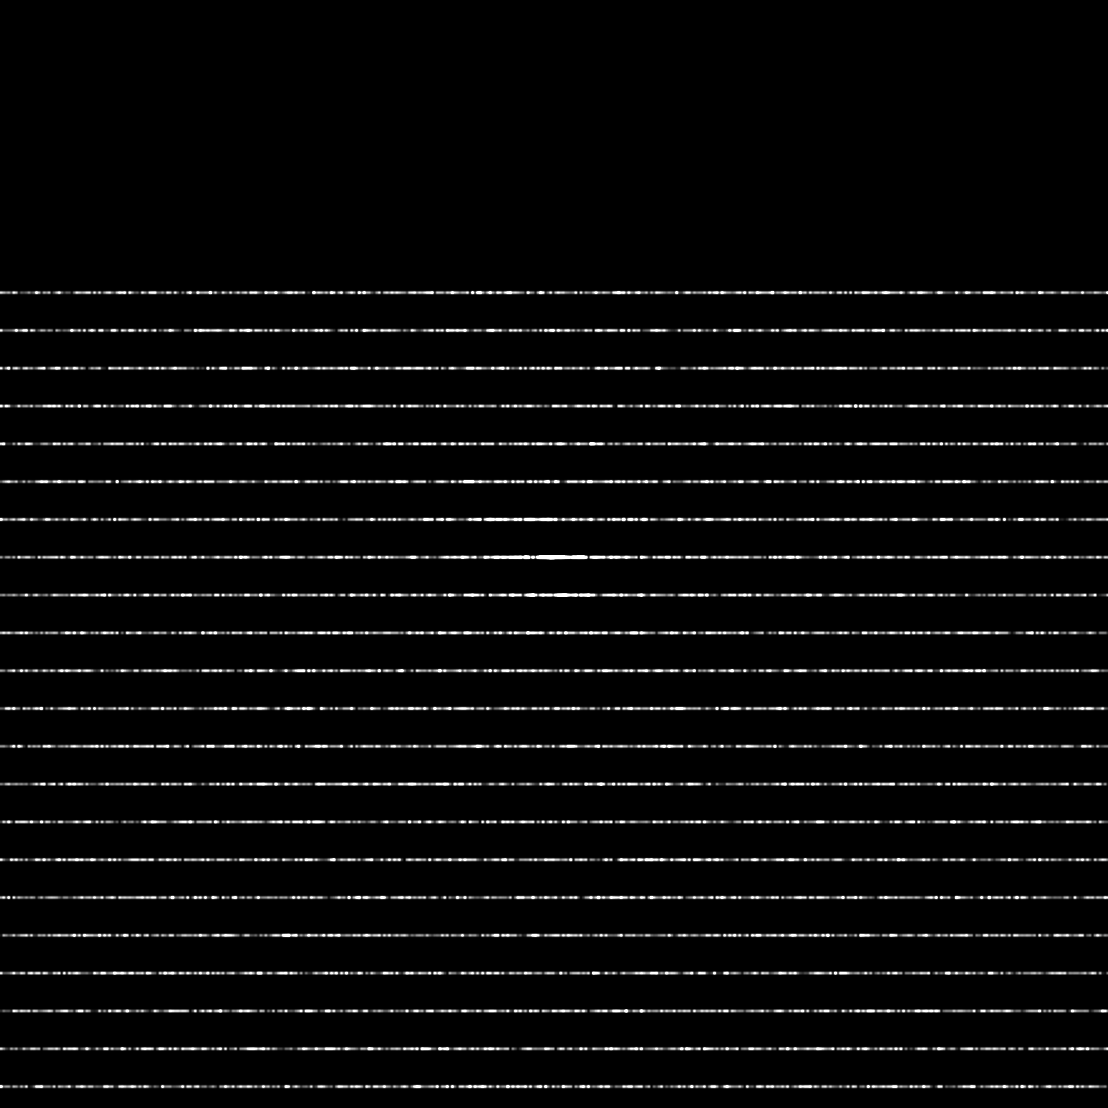
\includegraphics[width=.10\textwidth]{figures/ksp_dir-2_coil-1_shot-0.png}};
		\node[inner sep=0pt] (ksp-Shot0-dir1) at (12.50, 0.20)
		{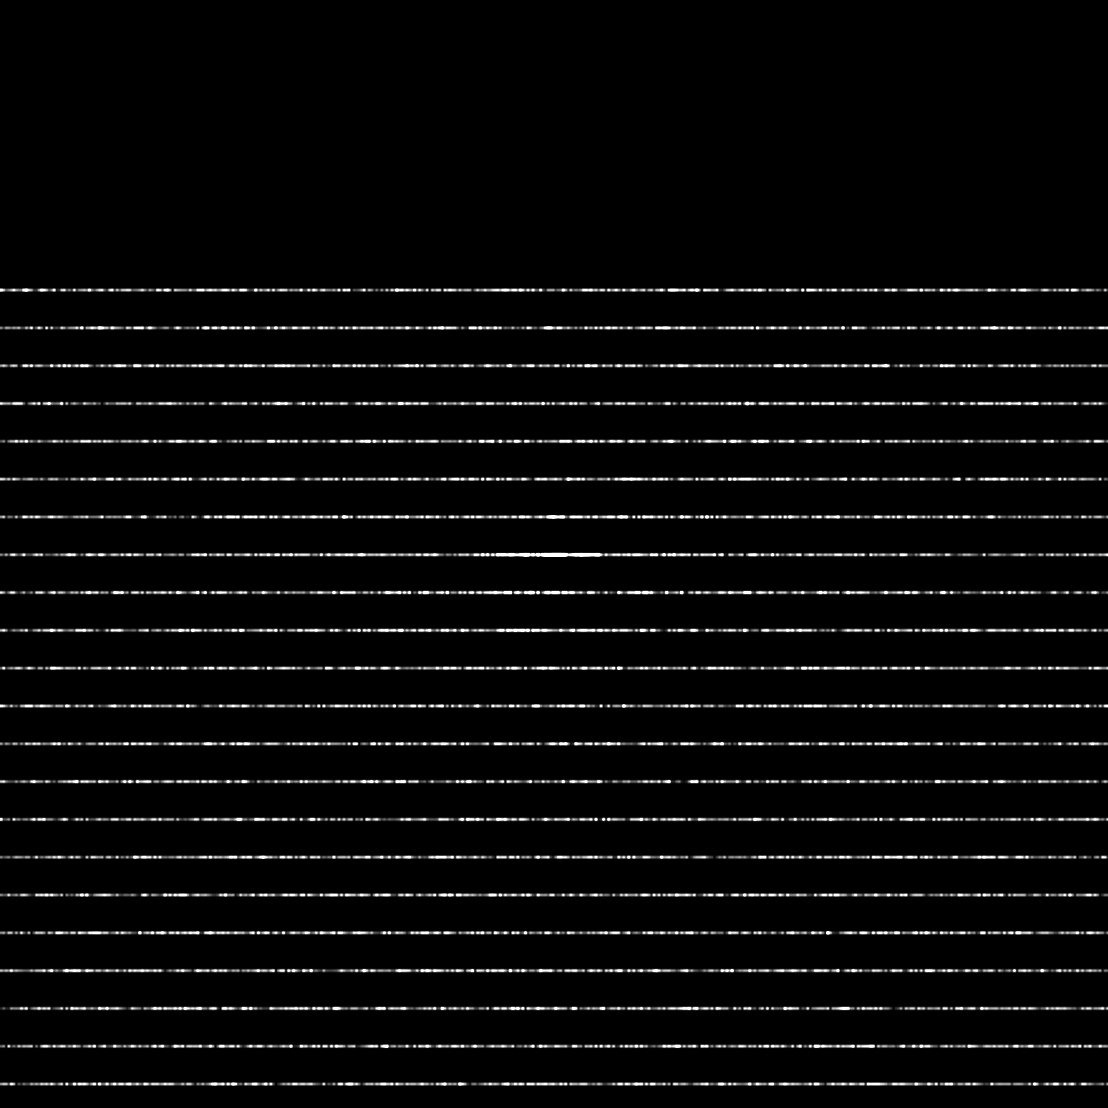
\includegraphics[width=.10\textwidth]{figures/ksp_dir-1_coil-1_shot-0.png}};

		\fill (13.7, 0.55) circle (1pt);
		\fill (13.8, 0.55) circle (1pt);
		\fill (13.9, 0.55) circle (1pt);

		\node[inner sep=0pt] (ksp-Shot4-dir0) at (15.15, 0.65)
		{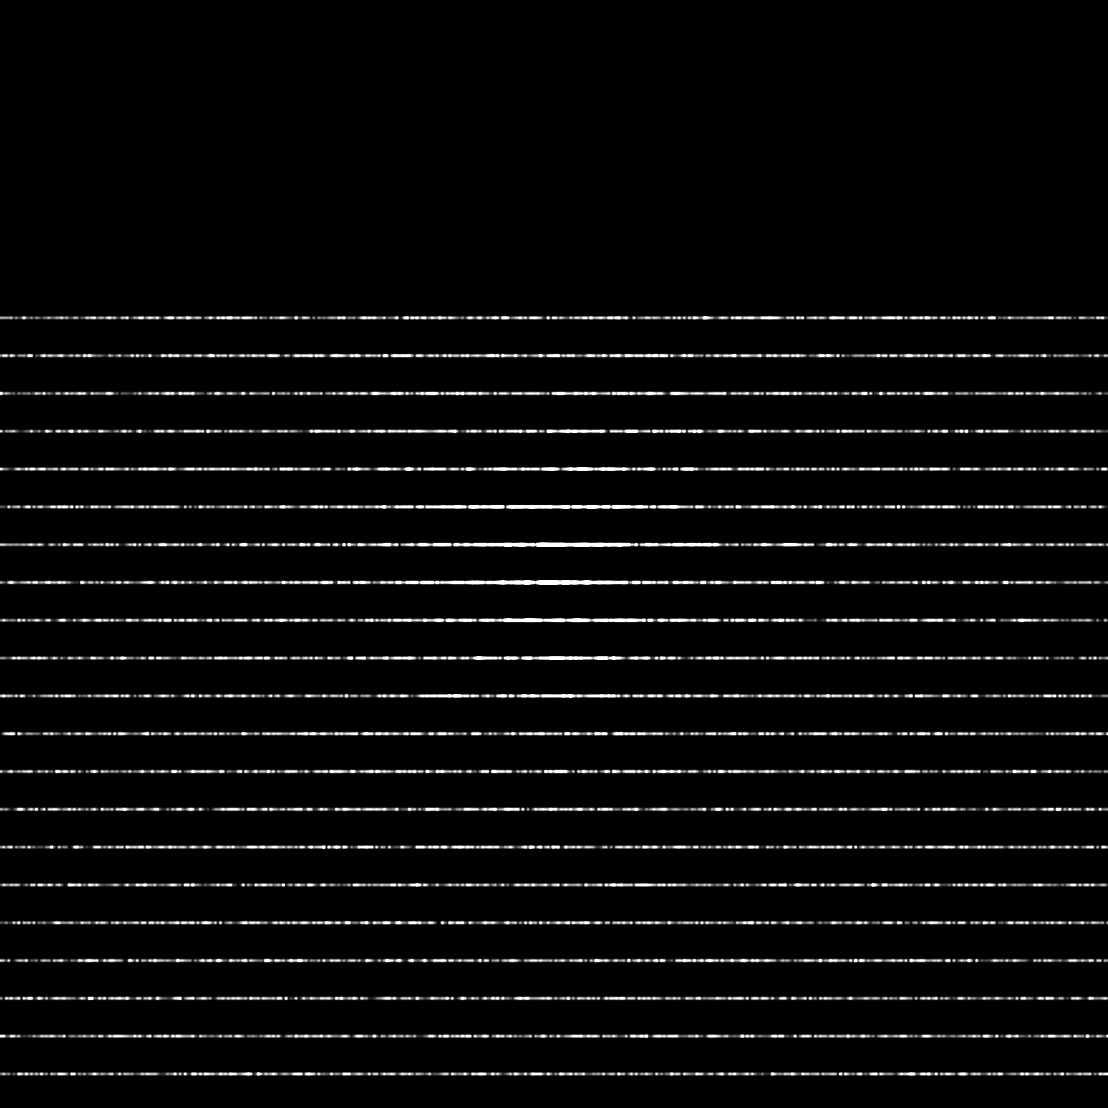
\includegraphics[width=.10\textwidth]{figures/ksp_dir-0_coil-1_shot-4.png}};
		\node[inner sep=0pt] (ksp-Shot4-dir3) at (15.00, 0.50)
		{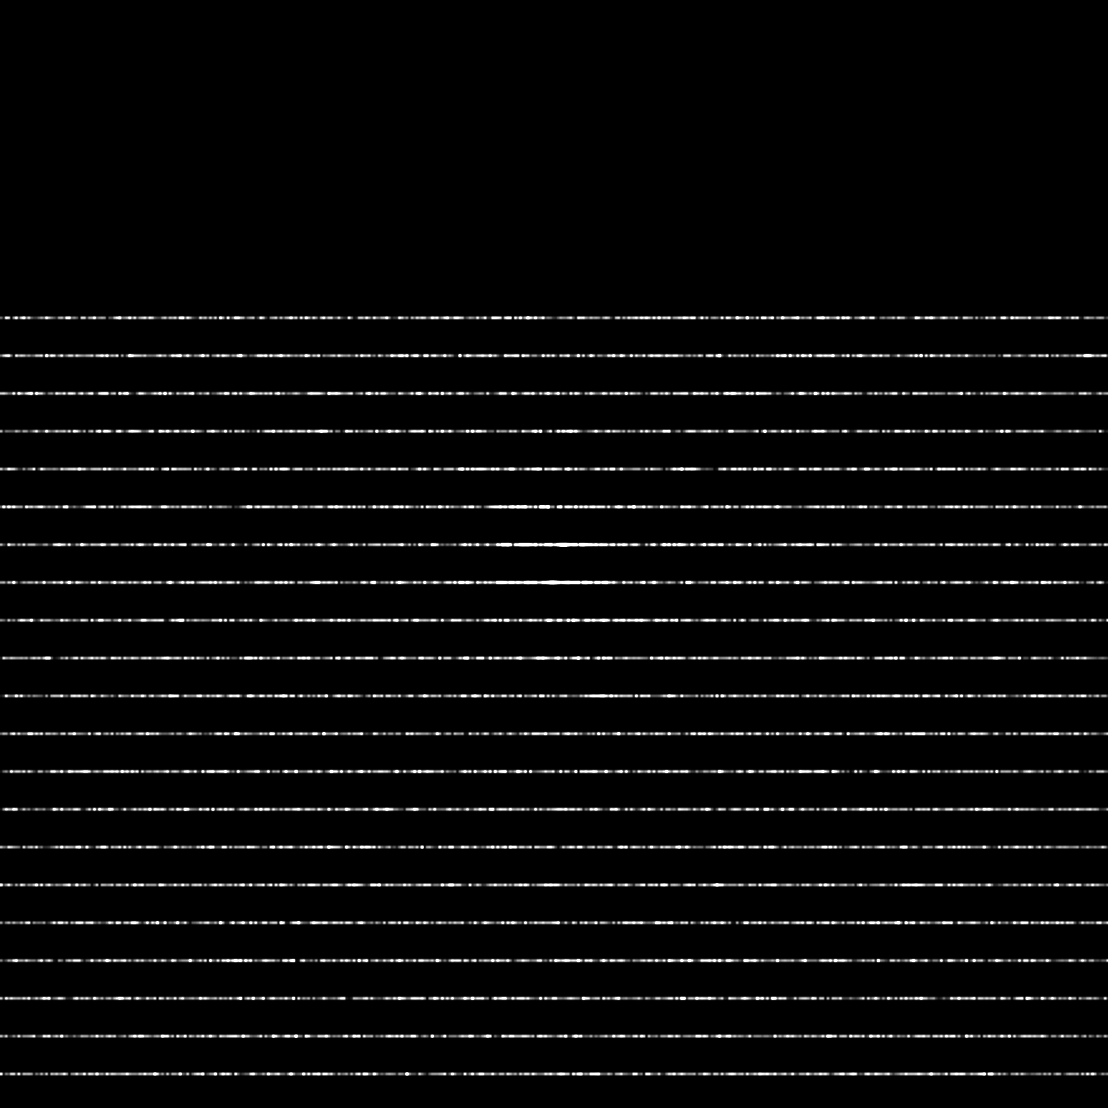
\includegraphics[width=.10\textwidth]{figures/ksp_dir-3_coil-1_shot-4.png}};
		\node[inner sep=0pt] (ksp-Shot4-dir2) at (14.85, 0.35)
		{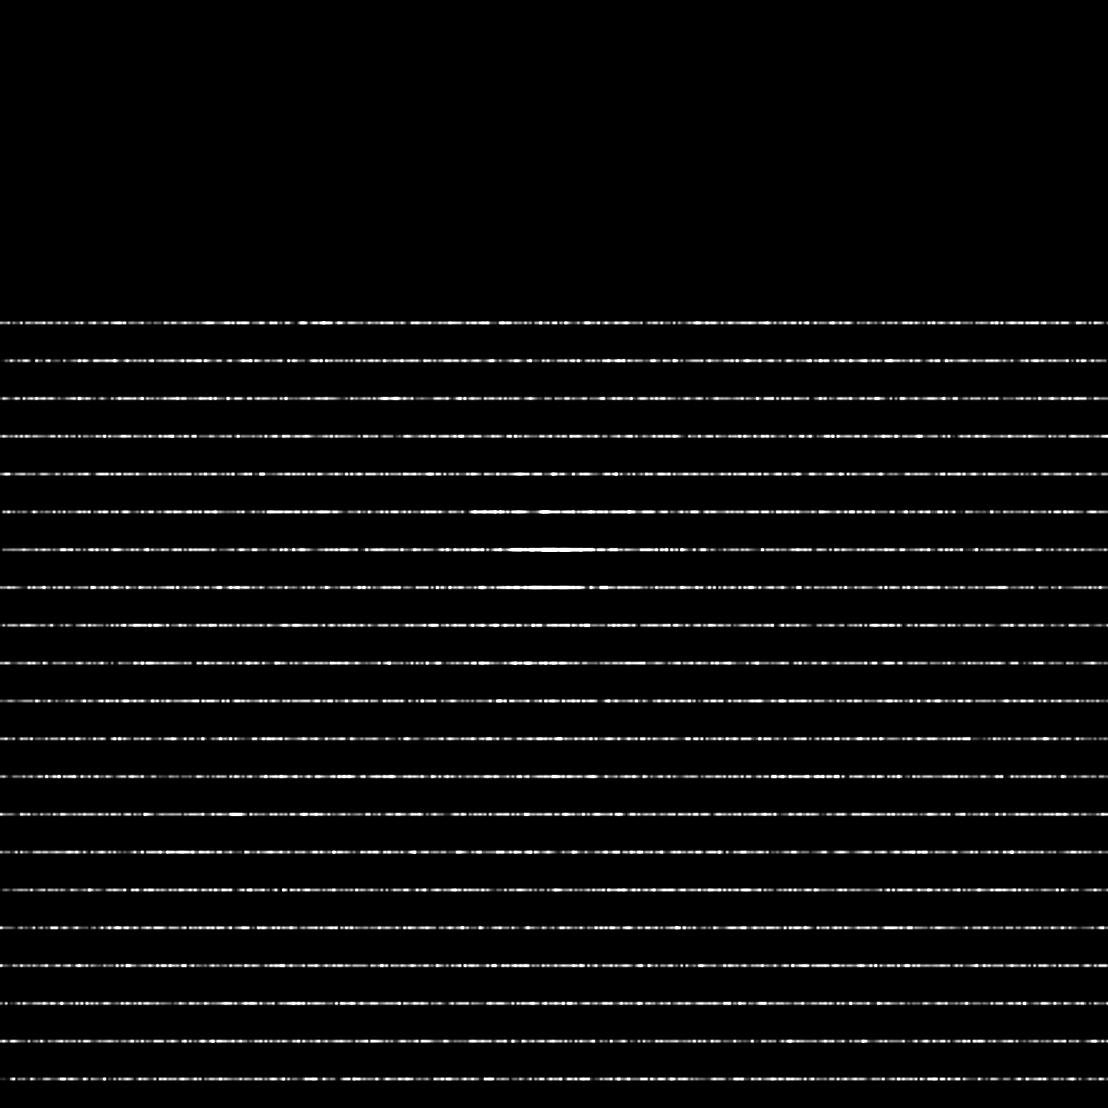
\includegraphics[width=.10\textwidth]{figures/ksp_dir-2_coil-1_shot-4.png}};
		\node[inner sep=0pt] (ksp-Shot4-dir1) at (14.70, 0.20)
		{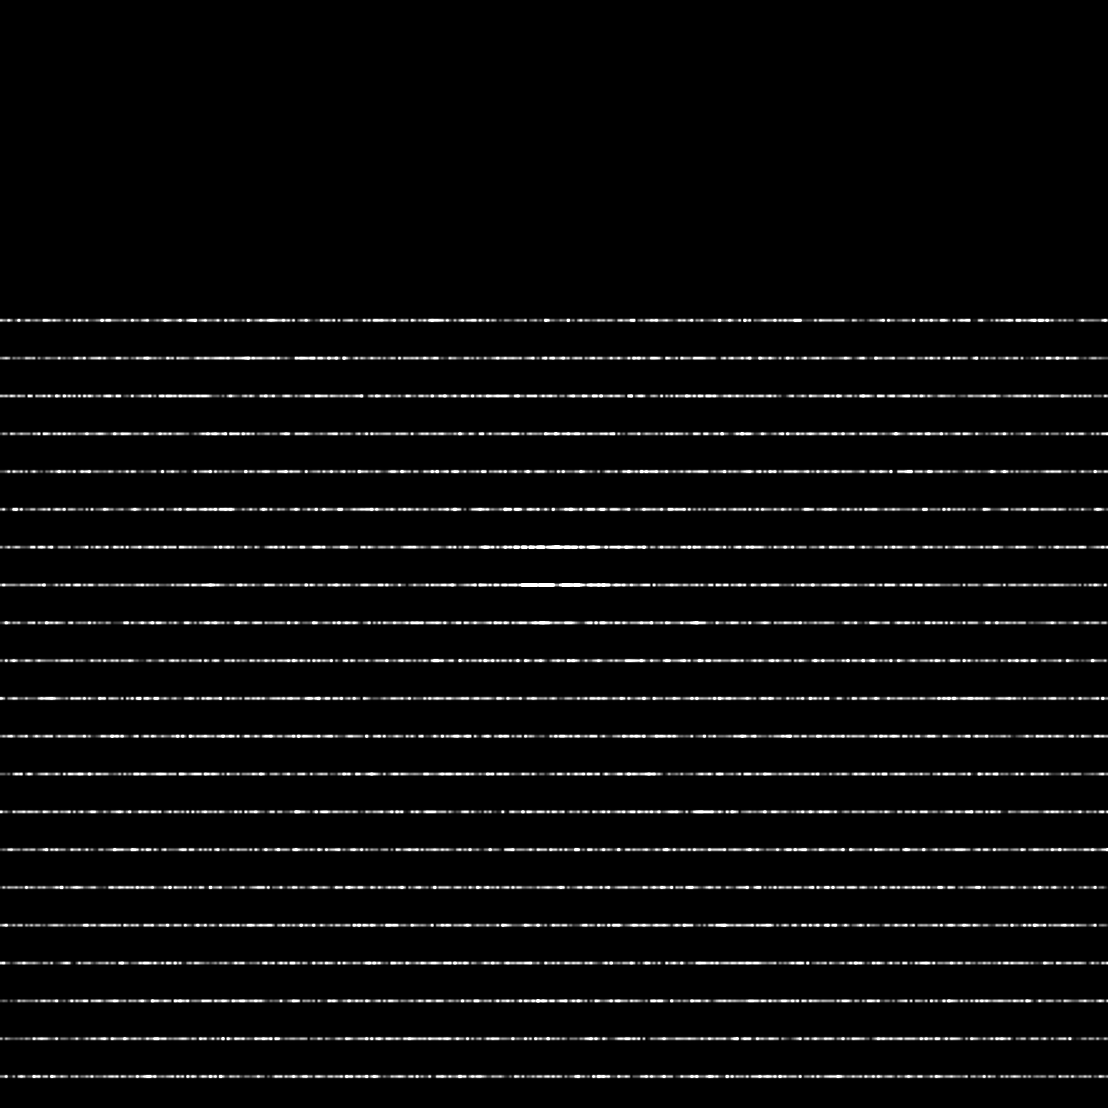
\includegraphics[width=.10\textwidth]{figures/ksp_dir-1_coil-1_shot-4.png}};

		\fill (12.9, -0.6) circle (1pt);
		\fill (12.9, -0.7) circle (1pt);
		\fill (12.9, -0.8) circle (1pt);

		\fill (15.1, -0.6) circle (1pt);
		\fill (15.1, -0.7) circle (1pt);
		\fill (15.1, -0.8) circle (1pt);

		\draw[->, line width=0.5pt] (11.5, 1) -- (11.5, 1.3);
		\node[font=\tiny] at (11.6, 1.3) {$c$};
		\draw[->, line width=0.5pt] (11.5, 1) -- (11.8, 1);
		\node[font=\tiny] at (11.9, 1) {$s$};
		\draw[->, line width=0.5pt] (11.5, 1) -- (11.3, 0.8);
		\node[font=\tiny] at (11.2, 0.8) {$q$};

		\node[font=\tiny] at (14.00, 1.6) {$k$-Space};

	\end{tikzpicture}
\end{document}
